\chapter{Hilbertov sistem aksiomov ravninske geometrije}

Ogledali si bomo Hilbertov sistem aksiomov ravninske geometrije, ki poskrbi za vse implicitne privzetke v Evklidovih aksiomih.

Kot nedefinirane pojme obravnavamo sledeče: \textit{točka}, \textit{premica}, \textit{leži na/leži med} in \textit{skladen}.

\begin{definicija}
    Za različni točki $A$ in  $B$ je \textbf{daljica} $AB$ množica, ki vsebuje točki $A$ in $B$ ter vse točke na premici $\overleftrightarrow{AB}$, ki ležijo med $A$ in $B$. Točki $A$ in $B$ imenujemo \textbf{krajišči} daljice $AB$.
\end{definicija}

\begin{definicija}
    Za poljubni različni točki $A$ in $B$ imenujemo množico vseh točk $P$, za katere je daljica $AP$ skladna z $AB$, \textbf{krožnica} s \textbf{središčem} $A$. Vsako daljico $AP$ imenujemo \textbf{polmer} krožnice.
\end{definicija}

\begin{definicija}
    \textbf{Poltrak} $\overrightarrow{AB}$ je naslednja množica točk na premici $\overleftrightarrow{AB}$: vsebuje vse točke na daljici $AB$ in tiste točke $C$ na $\overleftrightarrow{AB}$, za katere je $B$ med $A$ in $C$. Pravimo, da se poltrak $\overrightarrow{AB}$ \textbf{začne} v točki $A$ in da je \textbf{del} premice $\overleftrightarrow{AB}$.
\end{definicija}

\begin{definicija}
    Poltraka $\overrightarrow{AB}$ in $\overrightarrow{AC}$ sta $\textbf{nasprotna}$, če sta različna, se začneta v isti točki $A$ in sta del iste premice $\overleftrightarrow{AB}=\overleftrightarrow{AC}$
\end{definicija}

\begin{definicija}
    $\textbf{Kot z vrhom pri}~A$ je točka $A$ skupaj z dvema različnima poltrakoma $\overrightarrow{AB}$ in $\overrightarrow{AC}$, ki nista nasprotna. Poltraka imenujemo $\textbf{stranici}$ kota. Ta kot označimo z $\angle A$ ali $\angle BAC$ ali $\angle CAB$.
\end{definicija}

\begin{definicija}
    Če imata kota $\angle BAD$ in $\angle CAD$ skupno stranico $\overrightarrow{AD}$ in sta drugi stranici $\overrightarrow{AB}$ in $\overrightarrow{AC}$ nasprotna poltraka, imenujemo kota $\textbf{suplementarna}$.
\end{definicija}

\begin{definicija}
    Kot $\angle BAD$ je $\textbf{pravi kot}$, če ima skladen suplementaren kot.
\end{definicija}

\begin{definicija}
    Premici $p$ in $q$ sta $\textbf{vzporedni}$, če se ne sekata (tj. nimata skupnih točk). Oznaka $p\parallel q$.
\end{definicija}


\section*{Prvi Evklidov aksiom}

    \begin{aksiom}[E.1] 
        Za poljubni različni točki $A$ in $B$ obstaja natanko ena premica $p$, ki gre skozi $A$ in $B$.
    \end{aksiom}

        \begin{tikzpicture}
            % \clip (0,0) rectangle (14.000000,10.000000);
            {\footnotesize
            
            % Marking point A by circle
            \draw [line width=0.016cm] (2.000000,3.000000) circle (0.040000);%
            \draw (2.030000,2.970000) node [anchor=south east] { $A$ };%
            
            % Marking point B by circle
            \draw [line width=0.016cm] (4.000000,3.500000) circle (0.040000);%
            \draw (4.030000,3.470000) node [anchor=south east] { $B$ };%
            
            % Drawing line p
            \draw [line width=0.016cm] (1.000000,2.750000) -- (1.961194,2.990299);%
            \draw [line width=0.016cm] (2.038806,3.009701) -- (3.961194,3.490299);%
            \draw [line width=0.016cm] (4.038806,3.509701) -- (5.000000,3.750000);%
            }
        \end{tikzpicture}
        

\section{Aksiomi vsebovanosti}

        \begin{tikzpicture}
            % \clip (0,0) rectangle (14.000000,10.000000);
            {\footnotesize
            
            % Marking point A by circle
            \draw [line width=0.016cm] (2.000000,3.000000) circle (0.040000);%
            \draw (2.030000,2.970000) node [anchor=south east] { $A$ };%
            
            % Marking point B by circle
            \draw [line width=0.016cm] (4.000000,3.500000) circle (0.040000);%
            \draw (4.030000,3.470000) node [anchor=south east] { $B$ };%
            
            % Marking point C by circle
            \draw [line width=0.016cm] (5.000000,3.750000) circle (0.040000);%
            \draw (5.030000,3.720000) node [anchor=south east] { $C$ };%
            
            % Marking point D by circle
            \draw [line width=0.016cm] (3.000000,4.500000) circle (0.040000);%
            \draw (3.030000,4.470000) node [anchor=south east] { $D$ };%
            
            % Drawing line p
            \draw [line width=0.016cm] (1.000000,2.750000) -- (1.961194,2.990299);%
            \draw [line width=0.016cm] (2.038806,3.009701) -- (3.961194,3.490299);%
            \draw [line width=0.016cm] (4.038806,3.509701) -- (4.961194,3.740299);%
            \draw [line width=0.016cm] (5.038806,3.759701) -- (6.000000,4.000000);%
            }
        \end{tikzpicture}
    
    \begin{aksiom}[V.1]
        Za poljubni različni točki $A$ in $B$ obstaja natanko ena premica $p$, ki vsebuje $A$ in $B$.
    \end{aksiom}

    \begin{aksiom}[V.2]
        Na vsaki premici ležita vsaj dve različni točki.
    \end{aksiom}

    \begin{definicija}
        Točke imenujemo \textbf{kolinearne}, če ležijo na isti premici. Sicer rečemo, da so \textbf{nekolinearne}.
    \end{definicija}

    \begin{aksiom}[V.3]
        Obstajajo tri različne nekolinearne točke.
    \end{aksiom}

    \begin{trditev}
        ~
        \begin{enumerate}
            \item Če sta $p$ in $q$ različni premici, ki nista vzporedni, potem imata $p$ in $q$ natanko eno skupno točko.
            \item Obstajajo tri premice, take, da nobena točka ne leži na vseh treh.
                    Če bi obstajal $P$ na vseh premicah, bi vse premice sovpadale. 
            \item Za vsako premico $p$ obstaja vsaj ena točka, ki ni na $p$.
            \item Za vsako točko obstaja vsaj ena premica, ki je ne vsebuje.
            \item Skozi vsako točko gresta vsaj dve premici. \\
                \begin{tikzpicture}
                    % \clip (0,0) rectangle (14.000000,10.000000);
                    {\footnotesize
                    
                    % Drawing line p
                    \draw [line width=0.016cm] (1.000000,5.166667) -- (1.960544,5.006576);%
                    \draw [line width=0.016cm] (2.039456,4.993424) -- (4.960544,4.506576);%
                    \draw [line width=0.016cm] (5.039456,4.493424) -- (6.000000,4.333333);%
                    
                    % Drawing line s
                    \draw [line width=0.016cm] (4.666667,1.000000) -- (4.022188,1.966718);%
                    \draw [line width=0.016cm] (3.977812,2.033282) -- (2.022188,4.966718);%
                    \draw [line width=0.016cm] (1.977812,5.033282) -- (1.666667,5.500000);%
                    
                    % Drawing line r
                    \draw [line width=0.016cm] (3.600000,1.000000) -- (3.985144,1.962861);%
                    \draw [line width=0.016cm] (4.014856,2.037139) -- (4.985144,4.462861);%
                    \draw [line width=0.016cm] (5.014856,4.537139) -- (5.400000,5.500000);%
                    
                    % Marking point A by circle
                    \draw [line width=0.016cm] (2.000000,5.000000) circle (0.040000);%
                    \draw (1.970000,4.970000) node [anchor=south west] { $A$ };%
                    
                    % Marking point B by circle
                    \draw [line width=0.016cm] (5.000000,4.500000) circle (0.040000);%
                    \draw (4.970000,4.470000) node [anchor=south west] { $B$ };%
                    
                    % Marking point C by circle
                    \draw [line width=0.016cm] (4.000000,2.000000) circle (0.040000);%
                    \draw (3.970000,1.970000) node [anchor=south west] { $C$ };%
                    }
                \end{tikzpicture}
        \end{enumerate}


    \end{trditev}

    \noindent \textbf{MODELI}, ki ustrezajo tem aksiomom, glede na medsebojno lego premic:
    \begin{enumerate}
        \item MODEL SFERIČNE GEOMETRIJE: Imamo 3 točke ($A, B, C$), ki pripadajo premicam: $\left\{A, B\right\},$ $\left\{A, C\right\},$ $\left\{B, C\right\}$. Nobena premica si ni med seboj vzporedna.
        \item MODEL EVKLIDSKE GEOMETRIJE: Imamo 4 točke ($A, B, C, D$), ki pripadajo premicam: $\left\{A,B\right\},$ $\left\{A,C\right\},$ $\left\{A,D\right\}, \left\{B,C\right\}, \left\{B,D\right\}, \left\{C,D\right\}$. Skozi poljubno točko, ki ni na premici, poteka natanko ena vzporednica.
        \item MODEL HIPERBOLIČNE GEOMETRIJE: Imamo 5 točk ($A, B, C, D, E$), ki pripadajo premicam $\left\{A,B\right\},\left\{A,C\right\},\left\{A,D\right\},\left\{A,E\right\},\left\{B,C\right\},\left\{B,D\right\},\left\{B,E\right\},\left\{C,D\right\},\left\{C,E\right\},\left\{D,E\right\}$. Skozi poljubno točko, ki ni na premici, potekata natanko 2 vzporednici.
    \end{enumerate}

\section*{Drugi Evklidov aksiom}

    \begin{aksiom}[E.2]
        Za poljubni daljici $AB$ in $CD$ obstaja natanko ena točka $E$, da je $B$ med $A$ in $E$ ter je daljica $CD$ skladna z daljico $BE$.
    \end{aksiom}

        \begin{tikzpicture}
            % \clip (0,0) rectangle (14.000000,10.000000);
            {\footnotesize
            
            % Marking point A by circle
            \draw [line width=0.016cm] (2.000000,3.000000) circle (0.040000);%
            \draw (2.030000,2.970000) node [anchor=south east] { $A$ };%
            
            % Marking point B by circle
            \draw [line width=0.016cm] (4.000000,4.500000) circle (0.040000);%
            \draw (4.030000,4.470000) node [anchor=south east] { $B$ };%
            
            % Marking point C by circle
            \draw [line width=0.016cm] (3.000000,1.500000) circle (0.040000);%
            \draw (3.030000,1.470000) node [anchor=south east] { $C$ };%
            
            % Marking point D by circle
            \draw [line width=0.016cm] (5.000000,2.000000) circle (0.040000);%
            \draw (5.030000,1.970000) node [anchor=south east] { $D$ };%
            
            % Drawing line p
            \draw [line width=0.016cm] (6.666667,6.500000) -- (5.679739,5.759804);%
            \draw [line width=0.016cm] (5.618690,5.714017) -- (4.032000,4.524000);%
            \draw [line width=0.016cm] (3.968000,4.476000) -- (2.032000,3.024000);%
            \draw [line width=0.016cm] (1.968000,2.976000) -- (1.000000,2.250000);%
            
            % Drawing line s
            \draw [line width=0.016cm] (1.000000,1.000000) -- (2.961194,1.490299);%
            \draw [line width=0.016cm] (3.038806,1.509701) -- (4.961194,1.990299);%
            \draw [line width=0.016cm] (5.038806,2.009701) -- (7.000000,2.500000);%
            
            % Marking point E by circle
            \draw [line width=0.016cm] (5.656417,5.727307) circle (0.040000);%
            \draw (5.686417,5.697307) node [anchor=south east] { $E$ };%
            
            % Drawing segment B E
            \draw [line width=0.032cm] (4.032139,4.523813) -- (5.624278,5.703493);%
            
            % Drawing segment C D
            \draw [line width=0.032cm] (3.038806,1.509701) -- (4.961194,1.990299);%
            }
        \end{tikzpicture}
        

\section{Aksiomi vmesnosti}

    \begin{definicija}
        Simbol $A\ast B \ast C$ pomeni, da točka $B$ \textbf{leži med} točkama $A$ in $C$.
    \end{definicija}

    \begin{aksiom}[M.1]
        Če velja $A\ast B\ast C$, potem so $A$, $B$ in $C$ različne kolinearne točke in velja tudi $C\ast B\ast A$.
    \end{aksiom}

        \begin{tikzpicture}
            % \clip (0,0) rectangle (14.000000,10.000000);
            {\footnotesize
            
            % Marking point A by circle
            \draw [line width=0.016cm] (2.000000,3.000000) circle (0.040000);%
            \draw (2.030000,2.970000) node [anchor=south east] { $A$ };%
            
            % Marking point B by circle
            \draw [line width=0.016cm] (4.000000,4.500000) circle (0.040000);%
            \draw (4.030000,4.470000) node [anchor=south east] { $B$ };%
            
            % Marking point C by circle
            \draw [line width=0.016cm] (5.000000,5.250000) circle (0.040000);%
            \draw (5.030000,5.220000) node [anchor=south east] { $C$ };%
            
            % Drawing line p
            \draw [line width=0.016cm] (1.000000,2.250000) -- (1.968000,2.976000);%
            \draw [line width=0.016cm] (2.032000,3.024000) -- (3.968000,4.476000);%
            \draw [line width=0.016cm] (4.032000,4.524000) -- (4.968000,5.226000);%
            \draw [line width=0.016cm] (5.032000,5.274000) -- (5.500000,5.625000);%
            }
        \end{tikzpicture}
        

    \begin{aksiom}[M.2]
        Za poljubni različni točki $B$ in $D$ obstajajo točke $A$, $C$ in $E$ na premici $\overleftrightarrow{BD}$, da velja $A\ast B\ast D$, $B\ast C\ast D$ in $B\ast D\ast E$
    \end{aksiom}

        \begin{tikzpicture}
            % \clip (0,0) rectangle (14.000000,10.000000);
            {\footnotesize
            
            % Marking point A by circle
            \draw [line width=0.016cm] (2.000000,3.000000) circle (0.040000);%
            \draw (2.030000,2.970000) node [anchor=south east] { $A$ };%
            
            % Marking point B by circle
            \draw [line width=0.016cm] (3.500000,4.125000) circle (0.040000);%
            \draw (3.530000,4.095000) node [anchor=south east] { $B$ };%
            
            % Marking point C by circle
            \draw [line width=0.016cm] (4.000000,4.500000) circle (0.040000);%
            \draw (4.030000,4.470000) node [anchor=south east] { $C$ };%
            
            % Marking point D by circle
            \draw [line width=0.016cm] (5.000000,5.250000) circle (0.040000);%
            \draw (5.030000,5.220000) node [anchor=south east] { $D$ };%
            
            % Marking point E by circle
            \draw [line width=0.016cm] (5.500000,5.625000) circle (0.040000);%
            \draw (5.530000,5.595000) node [anchor=south east] { $E$ };%
            
            % Drawing line p
            \draw [line width=0.016cm] (1.000000,2.250000) -- (1.968000,2.976000);%
            \draw [line width=0.016cm] (2.032000,3.024000) -- (3.468000,4.101000);%
            \draw [line width=0.016cm] (3.532000,4.149000) -- (3.968000,4.476000);%
            \draw [line width=0.016cm] (4.032000,4.524000) -- (4.968000,5.226000);%
            \draw [line width=0.016cm] (5.032000,5.274000) -- (5.468000,5.601000);%
            \draw [line width=0.016cm] (5.532000,5.649000) -- (6.500000,6.375000);%
            }
        \end{tikzpicture}
        

    \begin{aksiom}[M.3]
        Če so $A$, $B$ in $C$ tri različne kolinearne točke, potem natanko ena od teh točk leži med preostalima.
    \end{aksiom}

    \begin{definicija}
        Naj bo $p$ premica in $A$, $B$ točki, ki ne ležita na $p$. Če je $A=B$ ali če daljica $AB$ nima skupnih točk s $p$, rečemo, da $A$ in $B$ \textbf{ležita na istem bregu} $p$. Če je $A\neq B$ in daljica $AB$ seka $p$, rečemo, da $A$ in $B$ \textbf{ležita na nasprotnih bregovih} $p$.
    \end{definicija}

        \begin{tikzpicture}
            % \clip (0,0) rectangle (14.000000,10.000000);
            {\footnotesize
            
            % Marking point p
            \draw (6.000000,3.500000) node [anchor=south east] { $p$ };%
            
            % Drawing line q
            \draw [line width=0.016cm] (1.000000,1.833333) -- (6.100000,3.533333);%
            
            % Marking point A by circle
            \draw [line width=0.016cm] (1.500000,3.000000) circle (0.040000);%
            \draw (1.530000,2.970000) node [anchor=south east] { $A$ };%
            
            % Marking point B by circle
            \draw [line width=0.016cm] (4.000000,3.500000) circle (0.040000);%
            \draw (4.030000,3.470000) node [anchor=south east] { $B$ };%
            
            % Drawing segment A B
            \draw [line width=0.016cm] (1.539223,3.007845) -- (3.960777,3.492155);%
            }
        \end{tikzpicture}
        \begin{tikzpicture}
            % \clip (0,0) rectangle (14.000000,10.000000);
            {\footnotesize
            
            % Marking point p
            \draw (6.000000,3.500000) node [anchor=south east] { $p$ };%
            
            % Drawing line q
            \draw [line width=0.016cm] (1.000000,1.833333) -- (6.100000,3.533333);%
            
            % Marking point A by circle
            \draw [line width=0.016cm] (1.500000,3.000000) circle (0.040000);%
            \draw (1.530000,2.970000) node [anchor=south east] { $A$ };%
            
            % Marking point B by circle
            \draw [line width=0.016cm] (4.000000,1.500000) circle (0.040000);%
            \draw (3.970000,1.470000) node [anchor=south west] { $B$ };%
            
            % Drawing segment A B
            \draw [line width=0.016cm] (1.534300,2.979420) -- (3.965700,1.520580);%
            }
        \end{tikzpicture}
            
        

    \begin{aksiom}[M.4]
        Za poljubno premico $p$ in poljubne točke $A$, $B$ in $C$, ki ne ležijo na $p$, velja:
        \begin{enumerate}[label=\roman*$)$]
            \item če sta $A$ in $B$ na istem bregu $p$ ter $B$ in $C$ na istem bregu $p$, potem sta tudi $A$ in $C$ na istem bregu $p$.
            \item če sta $A$ in $B$ na različnih bregovih $p$ ter $B$ in $C$ na različnih bregovih $p$, potem sta $A$ in $C$ na istem bregu $p$.
        \end{enumerate}
    \end{aksiom}

        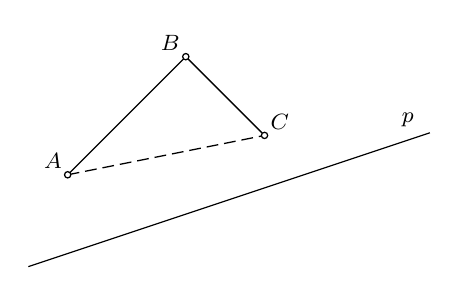
\begin{tikzpicture}
            % \clip (0,0) rectangle (14.000000,10.000000);
            {\footnotesize
            
            % Marking point p
            \draw (6.000000,3.500000) node [anchor=south east] { $p$ };%
            
            % Drawing line q
            \draw [line width=0.016cm] (1.000000,1.833333) -- (6.100000,3.533333);%
            
            % Marking point A by circle
            \draw [line width=0.016cm] (1.500000,3.000000) circle (0.040000);%
            \draw (1.530000,2.970000) node [anchor=south east] { $A$ };%
            
            % Marking point B by circle
            \draw [line width=0.016cm] (3.000000,4.500000) circle (0.040000);%
            \draw (3.030000,4.470000) node [anchor=south east] { $B$ };%
            
            % Marking point C by circle
            \draw [line width=0.016cm] (4.000000,3.500000) circle (0.040000);%
            \draw (3.970000,3.470000) node [anchor=south west] { $C$ };%
            
            % Drawing segment A B
            \draw [line width=0.016cm] (1.528284,3.028284) -- (2.971716,4.471716);%
            
            % Drawing segment B C
            \draw [line width=0.016cm] (3.028284,4.471716) -- (3.971716,3.528284);%
            
            % Drawing segment A C
            \draw [line width=0.016cm] (1.539223,3.007845) -- (1.647087,3.029417);%
            \draw [line width=0.016cm] (1.720631,3.044126) -- (1.867718,3.073544);%
            \draw [line width=0.016cm] (1.941261,3.088252) -- (2.088348,3.117670);%
            \draw [line width=0.016cm] (2.161892,3.132378) -- (2.308979,3.161796);%
            \draw [line width=0.016cm] (2.382523,3.176505) -- (2.529610,3.205922);%
            \draw [line width=0.016cm] (2.603153,3.220631) -- (2.750240,3.250048);%
            \draw [line width=0.016cm] (2.823784,3.264757) -- (2.970871,3.294174);%
            \draw [line width=0.016cm] (3.044415,3.308883) -- (3.191502,3.338300);%
            \draw [line width=0.016cm] (3.265045,3.353009) -- (3.412132,3.382426);%
            \draw [line width=0.016cm] (3.485676,3.397135) -- (3.632763,3.426553);%
            \draw [line width=0.016cm] (3.706307,3.441261) -- (3.853394,3.470679);%
            \draw [line width=0.016cm] (3.926937,3.485387) -- (3.960777,3.492155);%
            }
        \end{tikzpicture}
        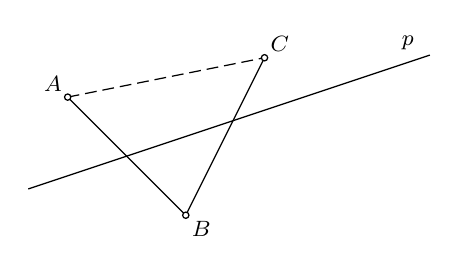
\begin{tikzpicture}
            % \clip (0,0) rectangle (14.000000,10.000000);
            {\footnotesize
            
            % Marking point p
            \draw (6.000000,3.500000) node [anchor=south east] { $p$ };%
            
            % Drawing line q
            \draw [line width=0.016cm] (1.000000,1.833333) -- (6.100000,3.533333);%
            
            % Marking point A by circle
            \draw [line width=0.016cm] (1.500000,3.000000) circle (0.040000);%
            \draw (1.530000,2.970000) node [anchor=south east] { $A$ };%
            
            % Marking point B by circle
            \draw [line width=0.016cm] (3.000000,1.500000) circle (0.040000);%
            \draw (2.970000,1.530000) node [anchor=north west] { $B$ };%
            
            % Marking point C by circle
            \draw [line width=0.016cm] (4.000000,3.500000) circle (0.040000);%
            \draw (3.970000,3.470000) node [anchor=south west] { $C$ };%
            
            % Drawing segment A B
            \draw [line width=0.016cm] (1.528284,2.971716) -- (2.971716,1.528284);%
            
            % Drawing segment B C
            \draw [line width=0.016cm] (3.017889,1.535777) -- (3.982111,3.464223);%
            
            % Drawing segment A C
            \draw [line width=0.016cm] (1.539223,3.007845) -- (1.647087,3.029417);%
            \draw [line width=0.016cm] (1.720631,3.044126) -- (1.867718,3.073544);%
            \draw [line width=0.016cm] (1.941261,3.088252) -- (2.088348,3.117670);%
            \draw [line width=0.016cm] (2.161892,3.132378) -- (2.308979,3.161796);%
            \draw [line width=0.016cm] (2.382523,3.176505) -- (2.529610,3.205922);%
            \draw [line width=0.016cm] (2.603153,3.220631) -- (2.750240,3.250048);%
            \draw [line width=0.016cm] (2.823784,3.264757) -- (2.970871,3.294174);%
            \draw [line width=0.016cm] (3.044415,3.308883) -- (3.191502,3.338300);%
            \draw [line width=0.016cm] (3.265045,3.353009) -- (3.412132,3.382426);%
            \draw [line width=0.016cm] (3.485676,3.397135) -- (3.632763,3.426553);%
            \draw [line width=0.016cm] (3.706307,3.441261) -- (3.853394,3.470679);%
            \draw [line width=0.016cm] (3.926937,3.485387) -- (3.960777,3.492155);%
            }
        \end{tikzpicture}
            
        


    \begin{posledica}
        Če sta $A$ in $B$ na različnih bregovih $p$ ter $B$ in $C$ na istem bregu $p$, potem sta $A$ in $C$ na različnih bregovih $p$.
    \end{posledica}

        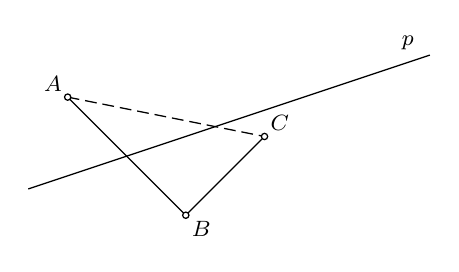
\begin{tikzpicture}
            % \clip (0,0) rectangle (14.000000,10.000000);
            {\footnotesize
            
            % Marking point p
            \draw (6.000000,3.500000) node [anchor=south east] { $p$ };%
            
            % Drawing line q
            \draw [line width=0.016cm] (1.000000,1.833333) -- (6.100000,3.533333);%
            
            % Marking point A by circle
            \draw [line width=0.016cm] (1.500000,3.000000) circle (0.040000);%
            \draw (1.530000,2.970000) node [anchor=south east] { $A$ };%
            
            % Marking point B by circle
            \draw [line width=0.016cm] (3.000000,1.500000) circle (0.040000);%
            \draw (2.970000,1.530000) node [anchor=north west] { $B$ };%
            
            % Marking point C by circle
            \draw [line width=0.016cm] (4.000000,2.500000) circle (0.040000);%
            \draw (3.970000,2.470000) node [anchor=south west] { $C$ };%
            
            % Drawing segment A B
            \draw [line width=0.016cm] (1.528284,2.971716) -- (2.971716,1.528284);%
            
            % Drawing segment B C
            \draw [line width=0.016cm] (3.028284,1.528284) -- (3.971716,2.471716);%
            
            % Drawing segment A C
            \draw [line width=0.016cm] (1.539223,2.992155) -- (1.647087,2.970583);%
            \draw [line width=0.016cm] (1.720631,2.955874) -- (1.867718,2.926456);%
            \draw [line width=0.016cm] (1.941261,2.911748) -- (2.088348,2.882330);%
            \draw [line width=0.016cm] (2.161892,2.867622) -- (2.308979,2.838204);%
            \draw [line width=0.016cm] (2.382523,2.823495) -- (2.529610,2.794078);%
            \draw [line width=0.016cm] (2.603153,2.779369) -- (2.750240,2.749952);%
            \draw [line width=0.016cm] (2.823784,2.735243) -- (2.970871,2.705826);%
            \draw [line width=0.016cm] (3.044415,2.691117) -- (3.191502,2.661700);%
            \draw [line width=0.016cm] (3.265045,2.646991) -- (3.412132,2.617574);%
            \draw [line width=0.016cm] (3.485676,2.602865) -- (3.632763,2.573447);%
            \draw [line width=0.016cm] (3.706307,2.558739) -- (3.853394,2.529321);%
            \draw [line width=0.016cm] (3.926937,2.514613) -- (3.960777,2.507845);%
            }
        \end{tikzpicture}
        
        \begin{dokaz}
            \\Dokaz naredimo s protislovjem: 
                Denimo, da sta $A$ in $C$ na istem bregu premice $p$. Potem sta $B$ in $C$ na istem bregu in $C$ in $A$ na istem bregu premice $p$. 
                Po Aksiomu (M.4) sledi: $A$ in $B$ sta na istem bregu premice $p$. To pa je protislovje.
        \end{dokaz}

    \begin{definicija}
        \textbf{Breg premice} $p$ ali \textbf{polravnina omejena s premico} $p$ je množica vseh točk, ki ležijo na istem bregu kot neka točka, ki ne leži na $p$.
    \end{definicija}

    \begin{trditev}
        Vsaka premica omejuje natanko dve polravnini. Ti polravnini nimata skupnih točk.
    \end{trditev}

        \begin{dokaz}
            \\
            \begin{tikzpicture}
                % \clip (0,0) rectangle (14.000000,10.000000);
                {\footnotesize
                
                % Drawing line q
                \draw [line width=0.016cm] (1.000000,2.836117) -- (2.480555,3.054543);%
                \draw [line width=0.016cm] (2.559699,3.066219) -- (6.000000,3.573765);%
                
                % Drawing line A C
                \draw [line width=0.016cm] (1.833333,1.000000) -- (1.987351,1.462053);%
                \draw [line width=0.016cm] (2.012649,1.537947) -- (2.507478,3.022434);%
                \draw [line width=0.016cm] (2.532776,3.098328) -- (2.987351,4.462053);%
                \draw [line width=0.016cm] (3.012649,4.537947) -- (3.166667,5.000000);%
                
                % Marking point A by circle
                \draw [line width=0.016cm] (3.000000,4.500000) circle (0.040000);%
                \draw (3.030000,4.470000) node [anchor=south east] { $A$ };%
                
                % Marking point B by circle
                \draw [line width=0.016cm] (2.520127,3.060381) circle (0.040000);%
                \draw (2.550127,3.030381) node [anchor=south east] { $B$ };%
                
                % Marking point C by circle
                \draw [line width=0.016cm] (2.000000,1.500000) circle (0.040000);%
                \draw (2.030000,1.470000) node [anchor=south east] { $C$ };%
                
                % Marking point p
                \draw (5.500000,3.500000) node [anchor=south east] { $p$ };%
                }
            \end{tikzpicture}
            \\ Obstajata natanko dva bregova premice $p$. Da ni več kot dveh bregov sledi iz Aksioma (M.4).
        \end{dokaz}

    \begin{trditev}
        ~
        \begin{enumerate}[label=\arabic*$)$]
            \item Če velja $A\ast B\ast C$ in $A\ast C\ast D$, potem velja $B\ast C\ast D$ in $A\ast B\ast D$.
            \item Če velja $A\ast B\ast C$ in $B\ast C\ast D$, potem velja $A\ast B\ast D$ in $A\ast C\ast D$.
        \end{enumerate}
    \end{trditev}

        \begin{dokaz}
            \\ Dokaz točke $1)$ za $B\ast C\ast D$: \\
                Po predpostavki vse točke ležijo na premici $\overleftrightarrow{AC}$ in zato so kolinearne.
                $A$, $B$ in $C$ so različne točke; $A$, $C$ in $D$ so tudi medsebojno različne.
                Če $B=D$, bi veljalo $A\ast B\ast C$ in $A\ast C\ast B$, kar je protislovje. (Velja natanko ena izmed možnosti.)
                \\
                \dashuline{$B\ast C\ast D$} \\
                    \begin{tikzpicture}
                        % \clip (0,0) rectangle (14.000000,10.000000);
                        {\footnotesize
                        
                        % Drawing line p
                        \draw [line width=0.016cm] (1.000000,1.500000) -- (1.964223,1.982111);%
                        \draw [line width=0.016cm] (2.035777,2.017889) -- (2.964223,2.482111);%
                        \draw [line width=0.016cm] (3.035777,2.517889) -- (3.991293,2.995646);%
                        \draw [line width=0.016cm] (4.062847,3.031424) -- (4.964223,3.482111);%
                        \draw [line width=0.016cm] (5.035777,3.517889) -- (6.000000,4.000000);%
                        
                        % Drawing line s
                        \draw [line width=0.016cm] (3.708211,1.000000) -- (4.020814,2.974027);%
                        \draw [line width=0.016cm] (4.033326,3.053043) -- (4.164582,3.881897);%
                        \draw [line width=0.016cm] (4.177095,3.960913) -- (4.341642,5.000000);%
                        
                        % Marking point A by circle
                        \draw [line width=0.016cm] (2.000000,2.000000) circle (0.040000);%
                        \draw (2.030000,1.970000) node [anchor=south east] { $A$ };%
                        
                        % Marking point B by circle
                        \draw [line width=0.016cm] (3.000000,2.500000) circle (0.040000);%
                        \draw (3.030000,2.470000) node [anchor=south east] { $B$ };%
                        
                        % Marking point C by circle
                        \draw [line width=0.016cm] (4.027070,3.013535) circle (0.040000);%
                        \draw (4.057070,2.983535) node [anchor=south east] { $C$ };%
                        
                        % Marking point D by circle
                        \draw [line width=0.016cm] (5.000000,3.500000) circle (0.040000);%
                        \draw (5.030000,3.470000) node [anchor=south east] { $D$ };%
                        
                        % Marking point E by circle
                        \draw [line width=0.016cm] (4.170838,3.921405) circle (0.040000);%
                        \draw (4.200838,3.891405) node [anchor=south east] { $E$ };%
                        }
                    \end{tikzpicture}
                    
                \noindent Izberimo $E\notin \overleftrightarrow{AC}$:
                \begin{itemize}
                    \item $AB$ ne seka $\overleftrightarrow{CE}$, saj bi sicer $\overleftrightarrow{AC}$ in $\overleftrightarrow{CE}$ imeli $2$ skupni točki (protislovje) $\Rightarrow$ $A$ in $B$ na istem bregu $\overleftrightarrow{CE}$
                    \item $AD$ seka $\overleftrightarrow{CE}$ v točki $C$ ($\Leftarrow A\ast C\ast D$) $\Rightarrow$ $A$ in $D$ na nasprotnih bregovih $\overleftrightarrow{CE}$
                \end{itemize}
                $\Rightarrow$ $B$ in $D$ na različnih bregovih $\overleftrightarrow{CE}$ \\
                $\Rightarrow$ daljica $BD$ seka $\overleftrightarrow{CE}$, ampak seka jo lahko le v $C$ \\
                $\Rightarrow$ ~ $B\ast C\ast D$ \\
                Podobno dokažemo za $A\ast B\ast D$ in točko $2)$.
        \end{dokaz}

    \begin{posledica}
        Če velja $C\ast A\ast B$ in je $p$ premica skozi $A$, $B$ in $C$, potem poljubna točka $D$ na $p$ leži bodisi na poltraku $\overrightarrow{AB}$ bodisi na nasprotnem poltraku $\overrightarrow{AC}$.
    \end{posledica}

    \begin{dokaz}
        \\ \begin{tikzpicture}
            % \clip (0,0) rectangle (14.000000,10.000000);
            {\footnotesize
            
            % Marking point p
            \draw (6.000000,3.500000) node [anchor=south west] { $p$ };%
            
            % Marking point q
            \draw (4.500000,4.000000) node [anchor=south east] { $q$ };%
            
            % Drawing line s
            \draw [line width=0.016cm] (1.000000,1.800000) -- (1.462861,1.985144);%
            \draw [line width=0.016cm] (1.537139,2.014856) -- (3.129528,2.651811);%
            \draw [line width=0.016cm] (3.203806,2.681522) -- (3.962861,2.985144);%
            \draw [line width=0.016cm] (4.037139,3.014856) -- (4.962861,3.385144);%
            \draw [line width=0.016cm] (5.037139,3.414856) -- (6.500000,4.000000);%
            
            % Drawing line r
            \draw [line width=0.016cm] (2.000000,1.500000) -- (3.138382,2.638382);%
            \draw [line width=0.016cm] (3.194951,2.694951) -- (5.500000,5.000000);%
            
            % Marking point A by circle
            \draw [line width=0.016cm] (3.166667,2.666667) circle (0.040000);%
            \draw (3.196667,2.636667) node [anchor=south east] { $A$ };%
            
            % Marking point B by circle
            \draw [line width=0.016cm] (4.000000,3.000000) circle (0.040000);%
            \draw (3.970000,3.030000) node [anchor=north west] { $B$ };%
            
            % Marking point C by circle
            \draw [line width=0.016cm] (1.500000,2.000000) circle (0.040000);%
            \draw (1.530000,1.970000) node [anchor=south east] { $C$ };%
            
            % Marking point D by circle
            \draw [line width=0.016cm] (5.000000,3.400000) circle (0.040000);%
            \draw (5.030000,3.370000) node [anchor=south east] { $D$ };%
            }
        \end{tikzpicture}
        \\ Premica $q$ deli ravnino na dva bregova/premico $p$ na dva dela. Potem sta točki $B$ in $C$ na različnih bregovih premice $q$. Točka $D$ leži na enem izmed bregov premice $q$. Torej $D$ leži na pripadajočem poltraku na premici $p$.
    \end{dokaz}    

    \begin{izrek}[Pasch]
        Naj bodo $A$, $B$ in $C$ nekolinearne točke in $p$ premica, ki seka $AB$ v neki točki, ki leži med $A$ in $B$. Potem $p$ seka bodisi $AC$ bodisi $BC$; če $C$ ne leži na $p$, potem $p$ ne seka obeh daljic $AC$ in $BC$.
    \end{izrek}

        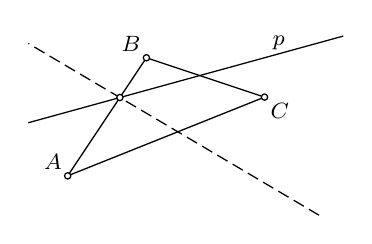
\begin{tikzpicture}
            % \clip (0,0) rectangle (14.000000,10.000000);
            {\footnotesize
            
            % Marking point p
            \draw (4.000000,3.500000) node [anchor=south west] { $p$ };%
            
            % Drawing line r
            \draw [line width=0.016cm] (4.692296,1.500000) -- (4.563157,1.576310);%
            \draw [line width=0.016cm] (4.498588,1.614465) -- (4.369449,1.690774);%
            \draw [line width=0.016cm] (4.304880,1.728929) -- (4.175741,1.805239);%
            \draw [line width=0.016cm] (4.111171,1.843394) -- (3.982033,1.919704);%
            \draw [line width=0.016cm] (3.917463,1.957859) -- (3.788325,2.034169);%
            \draw [line width=0.016cm] (3.723755,2.072323) -- (3.594616,2.148633);%
            \draw [line width=0.016cm] (3.530047,2.186788) -- (3.400908,2.263098);%
            \draw [line width=0.016cm] (3.336339,2.301253) -- (3.207200,2.377563);%
            \draw [line width=0.016cm] (3.142631,2.415718) -- (3.013492,2.492027);%
            \draw [line width=0.016cm] (2.948923,2.530182) -- (2.819784,2.606492);%
            \draw [line width=0.016cm] (2.755215,2.644647) -- (2.626076,2.720957);%
            \draw [line width=0.016cm] (2.561507,2.759112) -- (2.432368,2.835421);%
            \draw [line width=0.016cm] (2.367798,2.873576) -- (2.238660,2.949886);%
            \draw [line width=0.016cm] (2.128608,3.014917) -- (2.044952,3.064351);%
            \draw [line width=0.016cm] (1.980382,3.102506) -- (1.851243,3.178815);%
            \draw [line width=0.016cm] (1.786674,3.216970) -- (1.657535,3.293280);%
            \draw [line width=0.016cm] (1.592966,3.331435) -- (1.463827,3.407745);%
            \draw [line width=0.016cm] (1.399258,3.445900) -- (1.270119,3.522210);%
            \draw [line width=0.016cm] (1.205550,3.560364) -- (1.076411,3.636674);%
            \draw [line width=0.016cm] (1.011842,3.674829) -- (1.000000,3.681826);%
            
            % Drawing line s
            \draw [line width=0.016cm] (1.000000,2.674560) -- (2.124478,2.983956);%
            \draw [line width=0.016cm] (2.201612,3.005179) -- (5.000000,3.775147);%
            
            % Marking point A by circle
            \draw [line width=0.016cm] (1.500000,2.000000) circle (0.040000);%
            \draw (1.530000,1.970000) node [anchor=south east] { $A$ };%
            
            % Marking point B by circle
            \draw [line width=0.016cm] (2.500000,3.500000) circle (0.040000);%
            \draw (2.530000,3.470000) node [anchor=south east] { $B$ };%
            
            % Marking point C by circle
            \draw [line width=0.016cm] (4.000000,3.000000) circle (0.040000);%
            \draw (3.970000,3.030000) node [anchor=north west] { $C$ };%
            
            % Marking point D by circle
            \draw [line width=0.016cm] (2.163045,2.994568) circle (0.040000);%
            % \draw (2.193045,3.164568) node [anchor=south east] { $D$ };%
            
            % Drawing segment A B
            \draw [line width=0.016cm] (1.522188,2.033282) -- (2.140857,2.961286);%
            \draw [line width=0.016cm] (2.185233,3.027850) -- (2.477812,3.466718);%
            
            % Drawing segment A C
            \draw [line width=0.016cm] (1.537139,2.014856) -- (3.962861,2.985144);%
            
            % Drawing segment B C
            \draw [line width=0.016cm] (2.537947,3.487351) -- (3.962053,3.012649);%
            }
        \end{tikzpicture}

        \begin{dokaz}
            \\
            $1)$: $C\in p$ $\Rightarrow$ trditev drži \\
            $2)$: $C \notin p$: 
            Točki $A$ in $B$ ležita na različnih bregovih premice $p$, $C$ leži na enem izmed bregov premice $p$ istem kot $A$ ali $B$. 
            Na primer: $A$ in $C$ ležita na istem bregu $\Rightarrow$ $C$ in $B$ ležita na nasprotnih bregovih premice $p$ $\Rightarrow$ $CB$ seka $p$
        \end{dokaz}

    \begin{definicija}
        Točka $D$ leži \textbf{v notranjosti} kota $\angle CAB$, če $D$ leži na istem bregu premice $\overleftrightarrow{AC}$ kot $B$ in na istem bregu premice $\overleftrightarrow{AB}$ kot $C$.
    \end{definicija}

        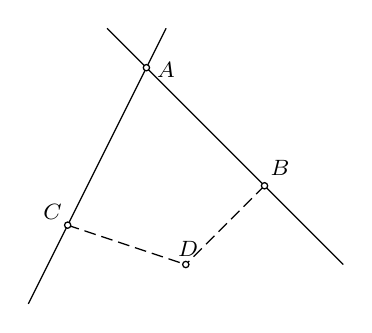
\begin{tikzpicture}
            % \clip (0,0) rectangle (14.000000,10.000000);
            {\footnotesize
            
            % Drawing line s
            \draw [line width=0.016cm] (2.000000,1.500000) -- (2.482111,2.464223);%
            \draw [line width=0.016cm] (2.517889,2.535777) -- (3.482111,4.464223);%
            \draw [line width=0.016cm] (3.517889,4.535777) -- (3.750000,5.000000);%
            
            % Drawing line r
            \draw [line width=0.016cm] (3.000000,5.000000) -- (3.471716,4.528284);%
            \draw [line width=0.016cm] (3.528284,4.471716) -- (4.971716,3.028284);%
            \draw [line width=0.016cm] (5.028284,2.971716) -- (6.000000,2.000000);%
            
            % Marking point A by circle
            \draw [line width=0.016cm] (3.500000,4.500000) circle (0.040000);%
            \draw (3.530000,4.470000) node [anchor=west] { $A$ };%
            
            % Marking point B by circle
            \draw [line width=0.016cm] (5.000000,3.000000) circle (0.040000);%
            \draw (4.970000,3.030000) node [anchor=south west] { $B$ };%
            
            % Marking point C by circle
            \draw [line width=0.016cm] (2.500000,2.500000) circle (0.040000);%
            \draw (2.530000,2.470000) node [anchor=south east] { $C$ };%
            
            % Marking point D by circle
            \draw [line width=0.016cm] (4.000000,2.000000) circle (0.040000);%
            \draw (4.030000,2.000000) node [anchor=south] { $D$ };%
            
            % Drawing segment B D
            \draw [line width=0.016cm] (4.971716,2.971716) -- (4.893934,2.893934);%
            \draw [line width=0.016cm] (4.840901,2.840901) -- (4.734835,2.734835);%
            \draw [line width=0.016cm] (4.681802,2.681802) -- (4.575736,2.575736);%
            \draw [line width=0.016cm] (4.522703,2.522703) -- (4.416637,2.416637);%
            \draw [line width=0.016cm] (4.363604,2.363604) -- (4.257538,2.257538);%
            \draw [line width=0.016cm] (4.204505,2.204505) -- (4.098439,2.098439);%
            \draw [line width=0.016cm] (4.045406,2.045406) -- (4.028284,2.028284);%
            
            % Drawing segment C D
            \draw [line width=0.016cm] (2.537947,2.487351) -- (2.642302,2.452566);%
            \draw [line width=0.016cm] (2.713454,2.428849) -- (2.855756,2.381415);%
            \draw [line width=0.016cm] (2.926907,2.357698) -- (3.069210,2.310263);%
            \draw [line width=0.016cm] (3.140361,2.286546) -- (3.282664,2.239112);%
            \draw [line width=0.016cm] (3.353815,2.215395) -- (3.496117,2.167961);%
            \draw [line width=0.016cm] (3.567269,2.144244) -- (3.709571,2.096810);%
            \draw [line width=0.016cm] (3.780722,2.073093) -- (3.923025,2.025658);%
            }
        \end{tikzpicture}
        

    \begin{trditev}
        Točka $D$ na premici $\overleftrightarrow{BC}$ leži v notranjosti kota $\angle CAB$ natanko tedaj, ko velja $B\ast D\ast C$.
    \end{trditev}

        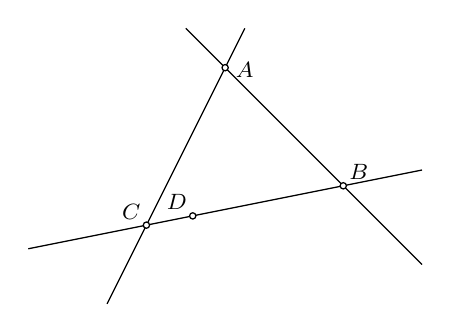
\begin{tikzpicture}
            % \clip (0,0) rectangle (14.000000,10.000000);
            {\footnotesize
            
            % Drawing line s
            \draw [line width=0.016cm] (2.000000,1.500000) -- (2.482111,2.464223);%
            \draw [line width=0.016cm] (2.517889,2.535777) -- (3.482111,4.464223);%
            \draw [line width=0.016cm] (3.517889,4.535777) -- (3.750000,5.000000);%
            
            % Drawing line r
            \draw [line width=0.016cm] (3.000000,5.000000) -- (3.471716,4.528284);%
            \draw [line width=0.016cm] (3.528284,4.471716) -- (4.971716,3.028284);%
            \draw [line width=0.016cm] (5.028284,2.971716) -- (6.000000,2.000000);%
            
            % Drawing line p
            \draw [line width=0.016cm] (1.000000,2.200000) -- (2.460777,2.492155);%
            \draw [line width=0.016cm] (2.539223,2.507845) -- (3.049097,2.609819);%
            \draw [line width=0.016cm] (3.127544,2.625509) -- (4.960777,2.992155);%
            \draw [line width=0.016cm] (5.039223,3.007845) -- (6.000000,3.200000);%
            
            % Marking point A by circle
            \draw [line width=0.016cm] (3.500000,4.500000) circle (0.040000);%
            \draw (3.530000,4.470000) node [anchor=west] { $A$ };%
            
            % Marking point B by circle
            \draw [line width=0.016cm] (5.000000,3.000000) circle (0.040000);%
            \draw (4.970000,2.970000) node [anchor=south west] { $B$ };%
            
            % Marking point C by circle
            \draw [line width=0.016cm] (2.500000,2.500000) circle (0.040000);%
            \draw (2.530000,2.470000) node [anchor=south east] { $C$ };%
            
            % Marking point D by circle
            \draw [line width=0.016cm] (3.088321,2.617664) circle (0.040000);%
            \draw (3.118321,2.587664) node [anchor=south east] { $D$ };%
            }
        \end{tikzpicture}
        

    \begin{definicija}
        Poltrak $\overrightarrow{AD}$ leži med poltrakoma $\overrightarrow{AC}$ in $\overrightarrow{AB}$, če $\overrightarrow{AC}$ in $\overrightarrow{AB}$ nista nasprotna poltraka in $D$ leži v notranjosti kota $\angle CAB$.
    \end{definicija}

        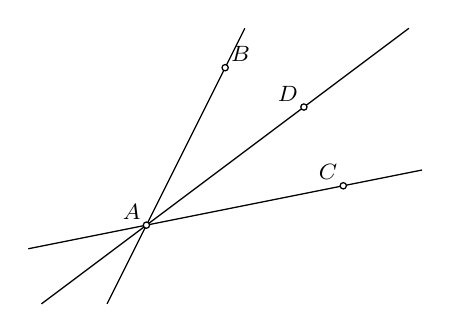
\begin{tikzpicture}
            % \clip (0,0) rectangle (14.000000,10.000000);
            {\footnotesize
            
            % Drawing line s
            \draw [line width=0.016cm] (1.000000,2.200000) -- (2.460777,2.492155);%
            \draw [line width=0.016cm] (2.539223,2.507845) -- (4.960777,2.992155);%
            \draw [line width=0.016cm] (5.039223,3.007845) -- (6.000000,3.200000);%
            
            % Drawing line r
            \draw [line width=0.016cm] (2.000000,1.500000) -- (2.482111,2.464223);%
            \draw [line width=0.016cm] (2.517889,2.535777) -- (3.482111,4.464223);%
            \draw [line width=0.016cm] (3.517889,4.535777) -- (3.750000,5.000000);%
            
            % Drawing line p
            \draw [line width=0.016cm] (1.166667,1.500000) -- (2.468000,2.476000);%
            \draw [line width=0.016cm] (2.532000,2.524000) -- (4.468000,3.976000);%
            \draw [line width=0.016cm] (4.532000,4.024000) -- (5.833333,5.000000);%
            
            % Marking point A by circle
            \draw [line width=0.016cm] (2.500000,2.500000) circle (0.040000);%
            \draw (2.530000,2.470000) node [anchor=south east] { $A$ };%
            
            % Marking point B by circle
            \draw [line width=0.016cm] (3.500000,4.500000) circle (0.040000);%
            \draw (3.470000,4.470000) node [anchor=south west] { $B$ };%
            
            % Marking point C by circle
            \draw [line width=0.016cm] (5.000000,3.000000) circle (0.040000);%
            \draw (5.030000,2.970000) node [anchor=south east] { $C$ };%
            
            % Marking point D by circle
            \draw [line width=0.016cm] (4.500000,4.000000) circle (0.040000);%
            \draw (4.530000,3.970000) node [anchor=south east] { $D$ };%
            }
        \end{tikzpicture}
        

    \begin{izrek}[o prečnici]
        Če $\overrightarrow{AD}$ leži med $\overrightarrow{AC}$ in $\overrightarrow{AB}$, potem $\overrightarrow{AD}$ seka daljico $BC$.
    \end{izrek}

        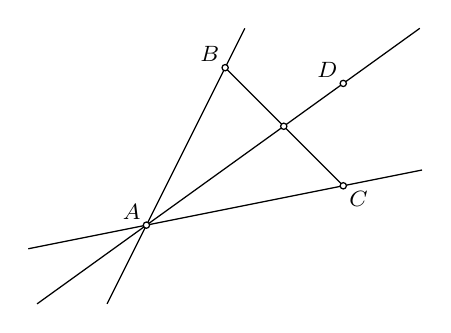
\begin{tikzpicture}
            % \clip (0,0) rectangle (14.000000,10.000000);
            {\footnotesize
            
            % Drawing line s
            \draw [line width=0.016cm] (1.000000,2.200000) -- (2.460777,2.492155);%
            \draw [line width=0.016cm] (2.539223,2.507845) -- (4.960777,2.992155);%
            \draw [line width=0.016cm] (5.039223,3.007845) -- (6.000000,3.200000);%
            
            % Drawing line r
            \draw [line width=0.016cm] (2.000000,1.500000) -- (2.482111,2.464223);%
            \draw [line width=0.016cm] (2.517889,2.535777) -- (3.482111,4.464223);%
            \draw [line width=0.016cm] (3.517889,4.535777) -- (3.750000,5.000000);%
            
            % Drawing line p
            \draw [line width=0.016cm] (1.111111,1.500000) -- (2.467539,2.476628);%
            \draw [line width=0.016cm] (2.532461,2.523372) -- (4.211725,3.732442);%
            \draw [line width=0.016cm] (4.276647,3.779186) -- (4.967539,4.276628);%
            \draw [line width=0.016cm] (5.032461,4.323372) -- (5.972222,5.000000);%
            
            % Marking point A by circle
            \draw [line width=0.016cm] (2.500000,2.500000) circle (0.040000);%
            \draw (2.530000,2.470000) node [anchor=south east] { $A$ };%
            
            % Marking point B by circle
            \draw [line width=0.016cm] (3.500000,4.500000) circle (0.040000);%
            \draw (3.530000,4.470000) node [anchor=south east] { $B$ };%
            
            % Marking point C by circle
            \draw [line width=0.016cm] (5.000000,3.000000) circle (0.040000);%
            \draw (4.970000,3.030000) node [anchor=north west] { $C$ };%
            
            % Marking point D by circle
            \draw [line width=0.016cm] (5.000000,4.300000) circle (0.040000);%
            \draw (5.030000,4.270000) node [anchor=south east] { $D$ };%
            
            % Marking point P by circle
            \draw [line width=0.016cm] (4.244186,3.755814) circle (0.040000);%
            
            % Drawing segment B C
            \draw [line width=0.016cm] (3.528284,4.471716) -- (4.215902,3.784098);%
            \draw [line width=0.016cm] (4.272470,3.727530) -- (4.971716,3.028284);%
            }
        \end{tikzpicture}
        

        \begin{dokaz}
            \\ $D$ je v notranjosti kota $\angle BAC$, tj. $D$ in $B$ sta na istem bregu premice $\overleftrightarrow{AC}$, $D$ in $C$ pa na istem bregu premice $\overleftrightarrow{AB}$
            \\ \dashuline{$\overleftrightarrow{AD}$ seka $BC$} 
            \\
                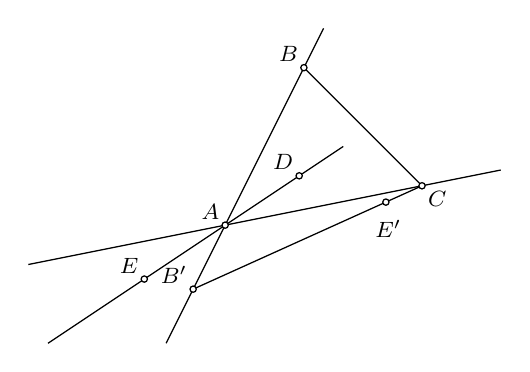
\begin{tikzpicture}
                    % \clip (0,0) rectangle (14.000000,10.000000);
                    {\footnotesize
                    
                    % Drawing segment B' C
                    \draw [line width=0.016cm] (3.130008,1.703576) -- (5.504788,2.776304);%
                    \draw [line width=0.016cm] (5.577695,2.809238) -- (5.963547,2.983533);%
                    
                    % Drawing line s
                    \draw [line width=0.016cm] (1.000000,2.000000) -- (3.460777,2.492155);%
                    \draw [line width=0.016cm] (3.539223,2.507845) -- (5.960777,2.992155);%
                    \draw [line width=0.016cm] (6.039223,3.007845) -- (7.000000,3.200000);%
                    
                    % Drawing line r
                    \draw [line width=0.016cm] (2.750000,1.000000) -- (3.075666,1.651332);%
                    \draw [line width=0.016cm] (3.111443,1.722886) -- (3.482111,2.464223);%
                    \draw [line width=0.016cm] (3.517889,2.535777) -- (4.482111,4.464223);%
                    \draw [line width=0.016cm] (4.517889,4.535777) -- (4.750000,5.000000);%
                    
                    % Drawing segment Q T
                    \draw [line width=0.016cm] (1.250000,1.000000) -- (2.439557,1.793038);%
                    \draw [line width=0.016cm] (2.506121,1.837414) -- (3.466718,2.477812);%
                    \draw [line width=0.016cm] (3.533282,2.522188) -- (4.406856,3.104571);%
                    \draw [line width=0.016cm] (4.473420,3.148947) -- (5.000000,3.500000);%
                    
                    % Marking point A by circle
                    \draw [line width=0.016cm] (3.500000,2.500000) circle (0.040000);%
                    \draw (3.530000,2.470000) node [anchor=south east] { $A$ };%
                    
                    % Marking point B by circle
                    \draw [line width=0.016cm] (4.500000,4.500000) circle (0.040000);%
                    \draw (4.530000,4.470000) node [anchor=south east] { $B$ };%
                    
                    % Marking point C by circle
                    \draw [line width=0.016cm] (6.000000,3.000000) circle (0.040000);%
                    \draw (5.970000,3.030000) node [anchor=north west] { $C$ };%
                    
                    % Marking point D by circle
                    \draw [line width=0.016cm] (4.440138,3.126759) circle (0.040000);%
                    \draw (4.470138,3.096759) node [anchor=south east] { $D$ };%
                    
                    % Marking point E by circle
                    \draw [line width=0.016cm] (2.472839,1.815226) circle (0.040000);%
                    \draw (2.502839,1.785226) node [anchor=south east] { $E$ };%
                    
                    % Marking point B' by circle
                    \draw [line width=0.016cm] (3.093554,1.687109) circle (0.040000);%
                    \draw (3.123554,1.657109) node [anchor=south east] { $B'$ };%
                    
                    % Marking point E' by circle
                    \draw [line width=0.016cm] (5.541242,2.792771) circle (0.040000);%
                    \draw (5.571242,2.662771) node [anchor=north] { $E'$ };%
                    
                    % Drawing segment B C
                    \draw [line width=0.016cm] (4.528284,4.471716) -- (5.971716,3.028284);%
                    }
                \end{tikzpicture}
            \\
            Denimo, da $\overleftrightarrow{AD}$  ne seka $BC$.
             $\Rightarrow$ $B$ in $C$ na istem bregu $\overleftrightarrow{AD}$
            \\ Naj bo $B' \in \overleftrightarrow{AB}$: $B\ast A\ast B'$ $\Rightarrow$ $B$ in $B'$ na nasprotnih bregovih premice $\overleftrightarrow{AD}$
            $\Rightarrow$ $B'$ in $C$ na nasprotnih bregovih premice $\overleftrightarrow{AD}$
            $\Rightarrow$ $B'C$ seka premico $\overleftrightarrow{AD}$ v neki točki $E$
            \\ Ker $B'C$ seka premico $\overleftrightarrow{AC}$ v točki $C$, daljica $B'E$ ne seka premice $\overleftrightarrow{AC}$ (sicer bi bilo $B'=A$)
            $\Rightarrow$ $B'$ in $E$ sta na istem bregu premice $\overleftrightarrow{AC}$
            $\Rightarrow$ $E$ in $B$ na nasprotnih bregovih
            $\Rightarrow$ $E$ in $D$ na nasprotnih bregovih premice $\overleftrightarrow{AC}$ 
            \\ Vemo: $B'C$ seka $\overleftrightarrow{AD}$ v $E$ in  $E$ in $D$ na nasprotnih bregovih $\overleftrightarrow{AC}$
            $\Rightarrow$ $\overleftrightarrow{ED}$ seka $\overleftrightarrow{AC}$ (nujno v $A$)
             $\Rightarrow$ $E\ast A\ast D$
             $\Rightarrow$ $E$ in $D$ na nasprotnih bregovih premice $\overleftrightarrow{AB}$ ter $D$ in $C$ na istem bregu premice  $\overleftrightarrow{AB}$
             $\Rightarrow$ $E$ in $C$ na nasprotnih bregovih premice $\overleftrightarrow{AB}$
            \\ $B'C$ seka $\overleftrightarrow{AB}$ v $B'$; $B'\ast E\ast C$ $\Rightarrow$ $EC$ seka $\overleftrightarrow{AB}$ 
             $\Rightarrow$ $E$ in $C$ sta na istem bregu premice. To pa je protislovje.
            \\ Sklep: $\overleftrightarrow{AD}$ seka $BC$ v točki $E$; $E \in \angle BAC$ $\Rightarrow$ $E \in \overleftrightarrow{AD}$
        \end{dokaz}

    \begin{definicija}
        Naj bodo $A$, $B$ in $C$ nekolinearne točke. 
        Rečemo, da $A$, $B$, $C$ določajo \textbf{trikotnik} $\triangle ABC$.
        \textbf{Notranjost} trikotnika $\triangle ABC$ je presek notranjosti njegovih kotov, tj. kotov ob ogliščih $A$, $B$ in $C$.
    \end{definicija}

        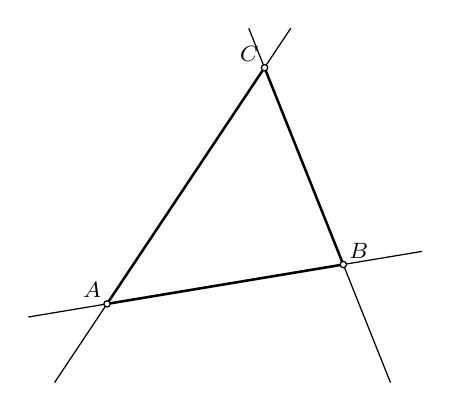
\begin{tikzpicture}
            % \clip (0,0) rectangle (14.000000,10.000000);
            {\footnotesize
            
            % Drawing line p
            \draw [line width=0.016cm] (1.000000,1.833333) -- (1.960544,1.993424);%
            \draw [line width=0.016cm] (2.039456,2.006576) -- (4.960544,2.493424);%
            \draw [line width=0.016cm] (5.039456,2.506576) -- (6.000000,2.666667);%
            
            % Drawing line s
            \draw [line width=0.016cm] (1.333333,1.000000) -- (1.977812,1.966718);%
            \draw [line width=0.016cm] (2.022188,2.033282) -- (3.977812,4.966718);%
            \draw [line width=0.016cm] (4.022188,5.033282) -- (4.333333,5.500000);%
            
            % Drawing line r
            \draw [line width=0.016cm] (5.600000,1.000000) -- (5.014856,2.462861);%
            \draw [line width=0.016cm] (4.985144,2.537139) -- (4.014856,4.962861);%
            \draw [line width=0.016cm] (3.985144,5.037139) -- (3.800000,5.500000);%
            
            % Marking point A by circle
            \draw [line width=0.016cm] (2.000000,2.000000) circle (0.040000);%
            \draw (2.030000,1.970000) node [anchor=south east] { $A$ };%
            
            % Marking point B by circle
            \draw [line width=0.016cm] (5.000000,2.500000) circle (0.040000);%
            \draw (4.970000,2.470000) node [anchor=south west] { $B$ };%
            
            % Marking point C by circle
            \draw [line width=0.016cm] (4.000000,5.000000) circle (0.040000);%
            \draw (4.030000,4.970000) node [anchor=south east] { $C$ };%
            
            % Drawing segment A B
            \draw [line width=0.032cm] (2.039456,2.006576) -- (4.960544,2.493424);%
            
            % Drawing segment A C
            \draw [line width=0.032cm] (2.022188,2.033282) -- (3.977812,4.966718);%
            
            % Drawing segment B C
            \draw [line width=0.032cm] (4.985144,2.537139) -- (4.014856,4.962861);%
            }
        \end{tikzpicture}
        


\section*{Tretji in četrti Evklidov aksiom}

    \begin{aksiom}[E.3]
        Za poljubni različni točki $A$ in $B$ obstaja krožnica s središčem $A$ in polmerom $AB$.
    \end{aksiom}

        \begin{tikzpicture}
            % \clip (0,0) rectangle (14.000000,10.000000);
            {\footnotesize
            
            % Marking point A by circle
            \draw [line width=0.016cm] (4.000000,3.000000) circle (0.040000);%
            \draw (4.030000,2.970000) node [anchor=south east] { $A$ };%
            
            % Marking point B by circle
            \draw [line width=0.016cm] (6.000000,3.500000) circle (0.040000);%
            \draw (5.970000,3.470000) node [anchor=south west] { $B$ };%
            
            % % Marking point P
            % \draw (4.228878,5.048808) node [anchor=south] { $P$ };%
            
            % Drawing circle p
            \draw [line width=0.016cm] (6.061553,3.000000) arc (0:12:2.061553 and 2.061553) -- (6.009324,3.461102);%
            \draw [line width=0.016cm] (5.989923,3.538710) -- (5.981692,3.568241) arc (16:360:2.061553 and 2.061553) --(6.061553,3.000000) arc (0:0:2.061553 and 2.061553);%
            
            % Drawing segment A B
            \draw [line width=0.016cm] (4.038806,3.009701) -- (5.961194,3.490299);%
            }
        \end{tikzpicture}
        
    \begin{aksiom}[E.4]
        Vsi pravi koti so skladni.
    \end{aksiom}

\section{Aksiomi skladnosti}

    \begin{aksiom}[S.1]
        Če sta $A$ in $B$ različni točki in $A'$ poljubna točka, potem na poljubnem poltraku $r$ z začetkom v $A'$ obstaja natanko ena točka $B'$, da velja $B'\neq A'$ in $AB\cong A'B'$.
    \end{aksiom}

        \begin{tikzpicture}
            % \clip (0,0) rectangle (14.000000,10.000000);
            {\footnotesize
            
            % Marking point A by circle
            \draw [line width=0.016cm] (1.500000,1.500000) circle (0.040000);%
            \draw (1.530000,1.470000) node [anchor=south east] { $A$ };%
            
            % Marking point B by circle
            \draw [line width=0.016cm] (3.000000,1.500000) circle (0.040000);%
            \draw (3.030000,1.470000) node [anchor=south east] { $B$ };%
            
            % Marking point A' by circle
            \draw [line width=0.016cm] (4.000000,1.500000) circle (0.040000);%
            \draw (4.030000,1.470000) node [anchor=south east] { $A'$ };%
            
            % Marking point B' by circle
            \draw [line width=0.016cm] (5.060660,2.560660) circle (0.040000);%
            \draw (5.090660,2.530660) node [anchor=south east] { $B'$ };%
            
            % Drawing segment A' G
            \draw [line width=0.016cm] (4.028284,1.528284) -- (5.032376,2.532376);%
            \draw [line width=0.016cm] (5.088944,2.588944) -- (6.000000,3.500000);%
            
            % Drawing segment A B
            \draw [line width=0.032cm] (1.540000,1.500000) -- (2.960000,1.500000);%
            
            % Drawing segment A' B'
            \draw [line width=0.032cm] (4.028284,1.528284) -- (5.032376,2.532376);%
            }
        \end{tikzpicture}
        

    \begin{aksiom}[S.2]
        Skladnost daljic je ekvivalenčna relacija.
    \end{aksiom}

    \begin{aksiom}[S.3]
        Če velja $A\ast B\ast C$, $A'\ast B'\ast C'$, $AB\cong A'B'$ in $BC\cong B'C'$, potem je $AC\cong A'C'$.
    \end{aksiom}

        \begin{tikzpicture}
            % \clip (0,0) rectangle (14.000000,10.000000);
            {\footnotesize
            
            % Marking point A by circle
            \draw [line width=0.016cm] (3.000000,1.500000) circle (0.040000);%
            \draw (3.030000,1.470000) node [anchor=south east] { $A$ };%
            
            % Marking point B by circle
            \draw [line width=0.016cm] (4.500000,1.500000) circle (0.040000);%
            \draw (4.530000,1.470000) node [anchor=south east] { $B$ };%
            
            % Marking point A' by circle
            \draw [line width=0.016cm] (2.000000,2.000000) circle (0.040000);%
            \draw (2.030000,1.970000) node [anchor=south east] { $A'$ };%
            
            % Marking point B' by circle
            \draw [line width=0.016cm] (3.060660,3.060660) circle (0.040000);%
            \draw (3.090660,3.030660) node [anchor=south east] { $B'$ };%
            
            % Marking point C by circle
            \draw [line width=0.016cm] (7.000000,1.500000) circle (0.040000);%
            \draw (7.030000,1.470000) node [anchor=south east] { $C$ };%
            
            % Marking point C' by circle
            \draw [line width=0.016cm] (4.828427,4.828427) circle (0.040000);%
            \draw (4.858427,4.798427) node [anchor=south east] { $C'$ };%
            
            % Drawing segment A'' G
            \draw [line width=0.016cm] (1.500000,1.500000) -- (1.971716,1.971716);%
            \draw [line width=0.016cm] (2.028284,2.028284) -- (3.032376,3.032376);%
            \draw [line width=0.016cm] (3.088944,3.088944) -- (4.800143,4.800143);%
            \draw [line width=0.016cm] (4.856711,4.856711) -- (5.500000,5.500000);%
            
            % Drawing segment F H
            \draw [line width=0.016cm] (2.000000,1.500000) -- (2.960000,1.500000);%
            \draw [line width=0.016cm] (3.040000,1.500000) -- (4.460000,1.500000);%
            \draw [line width=0.016cm] (4.540000,1.500000) -- (6.960000,1.500000);%
            \draw [line width=0.016cm] (7.040000,1.500000) -- (7.500000,1.500000);%
            
            % Drawing segment A B
            \draw [line width=0.032cm] (3.040000,1.500000) -- (4.460000,1.500000);%
            
            % Drawing segment A' B'
            \draw [line width=0.032cm] (2.028284,2.028284) -- (3.032376,3.032376);%
            
            % Drawing segment B C
            \draw [line width=0.032cm] (4.540000,1.500000) -- (4.650000,1.500000);%
            \draw [line width=0.032cm] (4.725000,1.500000) -- (4.875000,1.500000);%
            \draw [line width=0.032cm] (4.950000,1.500000) -- (5.100000,1.500000);%
            \draw [line width=0.032cm] (5.175000,1.500000) -- (5.325000,1.500000);%
            \draw [line width=0.032cm] (5.400000,1.500000) -- (5.550000,1.500000);%
            \draw [line width=0.032cm] (5.625000,1.500000) -- (5.775000,1.500000);%
            \draw [line width=0.032cm] (5.850000,1.500000) -- (6.000000,1.500000);%
            \draw [line width=0.032cm] (6.075000,1.500000) -- (6.225000,1.500000);%
            \draw [line width=0.032cm] (6.300000,1.500000) -- (6.450000,1.500000);%
            \draw [line width=0.032cm] (6.525000,1.500000) -- (6.675000,1.500000);%
            \draw [line width=0.032cm] (6.750000,1.500000) -- (6.900000,1.500000);%
            
            % Drawing segment B' C'
            \draw [line width=0.032cm] (3.088944,3.088944) -- (3.166726,3.166726);%
            \draw [line width=0.032cm] (3.219759,3.219759) -- (3.325825,3.325825);%
            \draw [line width=0.032cm] (3.378858,3.378858) -- (3.484924,3.484924);%
            \draw [line width=0.032cm] (3.537957,3.537957) -- (3.644023,3.644023);%
            \draw [line width=0.032cm] (3.697056,3.697056) -- (3.803122,3.803122);%
            \draw [line width=0.032cm] (3.856155,3.856155) -- (3.962221,3.962221);%
            \draw [line width=0.032cm] (4.015254,4.015254) -- (4.121320,4.121320);%
            \draw [line width=0.032cm] (4.174353,4.174353) -- (4.280419,4.280419);%
            \draw [line width=0.032cm] (4.333452,4.333452) -- (4.439518,4.439518);%
            \draw [line width=0.032cm] (4.492551,4.492551) -- (4.598618,4.598617);%
            \draw [line width=0.032cm] (4.651651,4.651650) -- (4.757717,4.757716);%
            }
        \end{tikzpicture}
        

    \begin{aksiom}[S.4]
        Za dani kot $\angle CAB$ in dani poltrak $\overrightarrow{A'B'}$ obstaja natanko en poltrak $\overrightarrow{A'C'}$ na izbranem bregu $\overleftrightarrow{A'B'}$, da velja $\angle C'A'B'\cong \angle CAB$.
    \end{aksiom}

        \begin{tikzpicture}
            % \clip (0,0) rectangle (14.000000,10.000000);
            {\footnotesize
            
            % Marking point A by circle
            \draw [line width=0.016cm] (1.500000,1.500000) circle (0.040000);%
            \draw (1.530000,1.470000) node [anchor=south east] { $A$ };%
            
            % Marking point B by circle
            \draw [line width=0.016cm] (4.400769,1.500000) circle (0.040000);%
            \draw (4.430769,1.470000) node [anchor=south east] { $B$ };%
            
            % Marking point C by circle
            \draw [line width=0.016cm] (3.311022,2.545594) circle (0.040000);%
            \draw (3.341022,2.515594) node [anchor=south east] { $C$ };%
            
            % Marking point A' by circle
            \draw [line width=0.016cm] (6.000000,2.500000) circle (0.040000);%
            \draw (6.030000,2.470000) node [anchor=south east] { $A'$ };%
            
            % Marking point B' by circle
            \draw [line width=0.016cm] (8.499100,2.812387) circle (0.040000);%
            \draw (8.529100,2.782387) node [anchor=south east] { $B'$ };%
            
            % Marking point C' by circle
            \draw [line width=0.016cm] (7.136081,3.359991) circle (0.040000);%
            \draw (7.166081,3.329991) node [anchor=south east] { $C'$ };%
            
            % Marking point C'' by circle
            \draw [line width=0.016cm] (6.870489,2.132739) circle (0.040000);%
            \draw (6.840489,2.102739) node [anchor=south west] { $C''$ };%
            
            % Drawing segment A G
            \draw [line width=0.016cm] (1.540000,1.500000) -- (4.360769,1.500000);%
            \draw [line width=0.016cm] (4.440769,1.500000) -- (5.000000,1.500000);%
            
            % Drawing segment A H
            \draw [line width=0.016cm] (1.534641,1.520000) -- (3.276381,2.525594);%
            \draw [line width=0.016cm] (3.345663,2.565594) -- (4.012140,2.950384);%
            
            % Drawing segment A' F
            \draw [line width=0.016cm] (6.039691,2.504961) -- (8.459409,2.807426);%
            \draw [line width=0.016cm] (8.538791,2.817349) -- (10.000000,3.000000);%
            
            % Drawing segment A' I
            \draw [line width=0.016cm] (6.031893,2.524142) -- (7.104188,3.335849);%
            \draw [line width=0.016cm] (7.167974,3.384134) -- (8.008090,4.020085);%
            
            % Drawing segment A' I'
            \draw [line width=0.016cm] (6.036854,2.484451) -- (6.138203,2.441692);%
            \draw [line width=0.016cm] (6.207305,2.412538) -- (6.345508,2.354229);%
            \draw [line width=0.016cm] (6.414610,2.325075) -- (6.552813,2.266767);%
            \draw [line width=0.016cm] (6.621915,2.237613) -- (6.760118,2.179304);%
            \draw [line width=0.016cm] (6.829220,2.150150) -- (6.833635,2.148288);%
            \draw [line width=0.016cm] (6.907343,2.117190) -- (6.967423,2.091842);%
            \draw [line width=0.016cm] (7.036524,2.062688) -- (7.174728,2.004379);%
            \draw [line width=0.016cm] (7.243829,1.975225) -- (7.382033,1.916917);%
            \draw [line width=0.016cm] (7.451134,1.887763) -- (7.589338,1.829455);%
            \draw [line width=0.016cm] (7.658439,1.800300) -- (7.796642,1.741992);%
            \draw [line width=0.016cm] (7.865744,1.712838) -- (8.003947,1.654530);%
            \draw [line width=0.016cm] (8.073049,1.625376) -- (8.211252,1.567067);%
            \draw [line width=0.016cm] (8.280354,1.537913) -- (8.320477,1.520985);%
            }
        \end{tikzpicture}
        

    \begin{aksiom}[S.5]
        Skladnost kotov je ekvivalenčna relacija.
    \end{aksiom}

    \begin{definicija}
        Trikotnika $\triangle ABC$ in $\triangle A'B'C'$ sta \textbf{skladna}, če so skladne istoležne stranice in istoležni koti.
    \end{definicija}

    \begin{aksiom}[S.6 ali SKS]
        Če sta stranici in vmesni kot enega trikotnika skladni s stranicama in vmesnim kotom drugega trikotnika, potem sta trikotnika skladna.
    \end{aksiom}

    \begin{trditev}[I.4, SKS]
        Če za trikotnika velja, da imata skladen par stranic in skladna kota, ki ju ti stranici oklepata, potem sta skladna.
    \end{trditev}

        \begin{tikzpicture}
            % \clip (0,0) rectangle (14.000000,10.000000);
            {\footnotesize
            
            % Drawing segment A B
            \draw [line width=0.016cm] (1.540000,1.500000) -- (4.460000,1.500000);%
            
            % Drawing segment A C
            \draw [line width=0.016cm] (1.514856,1.537139) -- (2.485144,3.962861);%
            
            % Drawing segment B C
            \draw [line width=0.016cm] (4.475012,1.531235) -- (2.524988,3.968765);%
            
            % Drawing segment A' B'
            \draw [line width=0.016cm] (5.540000,1.500000) -- (8.460000,1.500000);%
            
            % Drawing segment A' C'
            \draw [line width=0.016cm] (5.514856,1.537139) -- (6.485144,3.962861);%
            
            % Drawing segment B' C'
            \draw [line width=0.016cm] (8.475012,1.531235) -- (6.524988,3.968765);%
            
            % Marking point A by circle
            \draw [line width=0.016cm] (1.500000,1.500000) circle (0.040000);%
            \draw (1.530000,1.470000) node [anchor=south east] { $A$ };%
            
            % Marking point B by circle
            \draw [line width=0.016cm] (4.500000,1.500000) circle (0.040000);%
            \draw (4.470000,1.470000) node [anchor=south west] { $B$ };%
            
            % Marking point C by circle
            \draw [line width=0.016cm] (2.500000,4.000000) circle (0.040000);%
            \draw (2.530000,3.970000) node [anchor=south east] { $C$ };%
            
            % Marking point A' by circle
            \draw [line width=0.016cm] (5.500000,1.500000) circle (0.040000);%
            \draw (5.530000,1.470000) node [anchor=south east] { $A'$ };%
            
            % Marking point B' by circle
            \draw [line width=0.016cm] (8.500000,1.500000) circle (0.040000);%
            \draw (8.470000,1.470000) node [anchor=south west] { $B'$ };%
            
            % Marking point C' by circle
            \draw [line width=0.016cm] (6.500000,4.000000) circle (0.040000);%
            \draw (6.530000,3.970000) node [anchor=south east] { $C'$ };%
            }
        \end{tikzpicture}
        
        \begin{dokaz}
            \\ Ideja je superpozicija, tj. $\triangle A'B'C'$ premaknemo na $\triangle ABC$. 
            Na $\overrightarrow{AB}$ izberemo točko $B''$, da je $AB''\cong A'B'\cong AB$ in zato je $B=B'$. 
            Od $\overrightarrow{AB}$ odmerimo kot $\angle A'$ na tistem bregu $\overleftrightarrow{AB}$, ki vsebuje točko $C$: to da kot $\angle BAC''\cong \angle B'A'C'\cong\angle BAC$ in sledi $\overrightarrow{AC''}=\overrightarrow{AC}$. 
            Če je $AC''\cong A'C'\cong AC$, potem sledi $C''=C$.
            Tako smo trikotnik $\triangle A'B'C'$ premaknili na trikotnik $\triangle ABC$ in zato preslikani trikotnik $\triangle A'B'C'$ sovpada s trikotnikom $\triangle ABC$. Torej se ta dva trikotnika ujemata v vseh stranicah in kotih.
        \end{dokaz}

    \begin{opomba}
        Ta argument temelji na tem, da lahko trikotnik skladno premaknemo, torej da obstaja izometrija ravnine, ki preslika en trikotnik na drugega. Ampak takih preslikav v naših aksiomih ni. Torej tega kriterija (SKS) iz naših aksiomov ni mogoče dokazati.
    \end{opomba}

    \begin{trditev}
        Naj bo dan $\triangle ABC$ in daljica $DE\cong AB$. Potem obstaja natanko ena točka $F$ na danem bregu $\overleftrightarrow{DE}$, da sta $\triangle ABC$ in $\triangle DEF$ skladna.
    \end{trditev}

        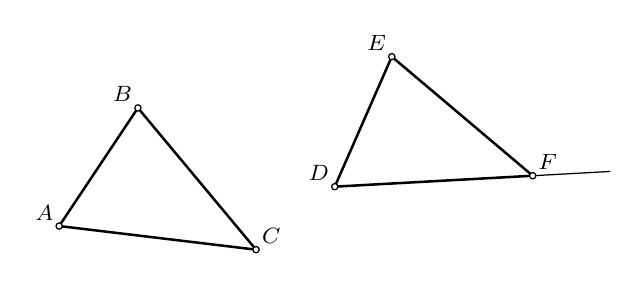
\begin{tikzpicture}
            % \clip (0,0) rectangle (14.000000,10.000000);
            {\footnotesize
            
            % Drawing segment D G
            \draw [line width=0.016cm] (5.039939,2.002203) -- (7.474175,2.136475);%
            \draw [line width=0.016cm] (7.554053,2.140881) -- (8.500000,2.193059);%
            
            % Marking point A by circle
            \draw [line width=0.016cm] (1.500000,1.500000) circle (0.040000);%
            \draw (1.530000,1.470000) node [anchor=south east] { $A$ };%
            
            % Marking point C by circle
            \draw [line width=0.016cm] (2.500000,3.000000) circle (0.040000);%
            \draw (2.530000,2.970000) node [anchor=south east] { $B$ };%
            
            % Marking point B by circle
            \draw [line width=0.016cm] (4.000000,1.200000) circle (0.040000);%
            \draw (3.970000,1.170000) node [anchor=south west] { $C$ };%
            
            % Marking point D by circle
            \draw [line width=0.016cm] (5.000000,2.000000) circle (0.040000);%
            \draw (5.030000,1.970000) node [anchor=south east] { $D$ };%
            
            % Marking point E by circle
            \draw [line width=0.016cm] (5.724336,3.650860) circle (0.040000);%
            \draw (5.754336,3.620860) node [anchor=south east] { $E$ };%
            
            % Marking point F by circle
            \draw [line width=0.016cm] (7.514114,2.138678) circle (0.040000);%
            \draw (7.484114,2.108678) node [anchor=south west] { $F$ };%
            
            % Drawing segment A B
            \draw [line width=0.032cm] (1.539715,1.495234) -- (3.960285,1.204766);%
            
            % Drawing segment A C
            \draw [line width=0.032cm] (1.522188,1.533282) -- (2.477812,2.966718);%
            
            % Drawing segment B C
            \draw [line width=0.032cm] (3.974393,1.230729) -- (2.525607,2.969271);%
            
            % Drawing segment D E
            \draw [line width=0.032cm] (5.016072,2.036629) -- (5.708264,3.614231);%
            
            % Drawing segment D F
            \draw [line width=0.032cm] (5.039939,2.002203) -- (7.474175,2.136475);%
            
            % Drawing segment E F
            \draw [line width=0.032cm] (5.754890,3.625044) -- (7.483559,2.164493);%
            }
        \end{tikzpicture}
        

    \begin{trditev}[I.5 -- Pons Asinorum ('oslovski most')]
        Če v $\triangle ABC$ velja $AB\cong AC$, potem je $\angle B\cong \angle C$.
    \end{trditev}

        \begin{tikzpicture}
            % \clip (0,0) rectangle (14.000000,10.000000);
            {\footnotesize
            
            % Drawing segment A B
            \draw [line width=0.016cm] (2.979420,3.965700) -- (1.520580,1.534300);%
            
            % Drawing segment A C
            \draw [line width=0.016cm] (3.020580,3.965700) -- (4.479420,1.534300);%
            
            % Drawing segment B C
            \draw [line width=0.016cm] (1.540000,1.500000) -- (4.460000,1.500000);%
            
            % Marking point A by circle
            \draw [line width=0.016cm] (3.000000,4.000000) circle (0.040000);%
            \draw (3.030000,3.970000) node [anchor=south east] { $A$ };%
            
            % Marking point B by circle
            \draw [line width=0.016cm] (1.500000,1.500000) circle (0.040000);%
            \draw (1.530000,1.470000) node [anchor=south east] { $B$ };%
            
            % Marking point C by circle
            \draw [line width=0.016cm] (4.500000,1.500000) circle (0.040000);%
            \draw (4.470000,1.470000) node [anchor=south west] { $C$ };%
            }
        \end{tikzpicture}
        
        \begin{dokaz}
            \\ Trikotnika $\triangle ABC$ in $\triangle ACB$ sta skladna po kriteriju SKS (S.6). 
            $\angle A$ je skupen in velja $AB\cong AC$, $AC\cong AB$ $\Rightarrow$ istoležni koti so skladni: $\angle B\cong \angle C$ in $\angle C\cong \angle B$.
        \end{dokaz}

    \begin{definicija}
        $AB<CD$ pomeni, da obstaja točka $E$ med $C$ in $D$, da velja $AB\cong CE$.
    \end{definicija}

        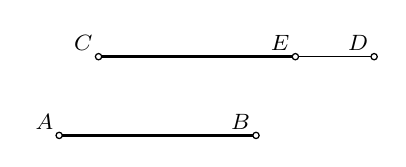
\begin{tikzpicture}
            % \clip (0,0) rectangle (14.000000,10.000000);
            {\footnotesize
            
            % Marking point A by circle
            \draw [line width=0.016cm] (1.500000,1.500000) circle (0.040000);%
            \draw (1.530000,1.470000) node [anchor=south east] { $A$ };%
            
            % Marking point B by circle
            \draw [line width=0.016cm] (4.000000,1.500000) circle (0.040000);%
            \draw (4.030000,1.470000) node [anchor=south east] { $B$ };%
            
            % Marking point C by circle
            \draw [line width=0.016cm] (2.000000,2.500000) circle (0.040000);%
            \draw (2.030000,2.470000) node [anchor=south east] { $C$ };%
            
            % Marking point D by circle
            \draw [line width=0.016cm] (5.500000,2.500000) circle (0.040000);%
            \draw (5.530000,2.470000) node [anchor=south east] { $D$ };%
            
            % Marking point E by circle
            \draw [line width=0.016cm] (4.500000,2.500000) circle (0.040000);%
            \draw (4.530000,2.470000) node [anchor=south east] { $E$ };%
            
            % Drawing segment C D
            \draw [line width=0.016cm] (2.040000,2.500000) -- (4.460000,2.500000);%
            \draw [line width=0.016cm] (4.540000,2.500000) -- (5.460000,2.500000);%
            
            % Drawing segment A B
            \draw [line width=0.032cm] (1.540000,1.500000) -- (3.960000,1.500000);%
            
            % Drawing segment C E
            \draw [line width=0.032cm] (2.040000,2.500000) -- (4.460000,2.500000);%
            }
        \end{tikzpicture}
        

    \begin{trditev}[Urejenost daljic]
        ~
        \begin{itemize}
            \item Velja natanko ena od možnosti: $AB<CD$, $AB\cong CD$ ali $AB>CD$. (Zakon trihotomije)
            \item Če je $AB<CD$ in $CD\cong EF$, potem je $AB<EF$.
            \item Če je $AB>CD$ in $CD\cong EF$, potem je $AB>EF$.
            \item Če je $AB<CD$ in $CD<EF$, potem je $AB<EF$.
        \end{itemize}
    \end{trditev}

    Analogna trditev velja za kote.

    \begin{trditev}
        Če sta kota skladna, potem sta tudi suplementarna kota skladna.
    \end{trditev}

        \begin{dokaz}
            \\ 
            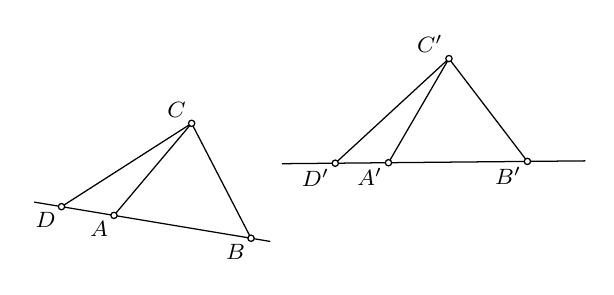
\begin{tikzpicture}
                % \clip (0,0) rectangle (14.000000,10.000000);
                {\footnotesize
                
                % Drawing segment F G
                \draw [line width=0.016cm] (4.648243,2.487314) -- (5.284123,2.493282);%
                \draw [line width=0.016cm] (5.364120,2.494033) -- (5.960002,2.499625);%
                \draw [line width=0.016cm] (6.039998,2.500375) -- (7.724176,2.516181);%
                \draw [line width=0.016cm] (7.804172,2.516931) -- (8.500000,2.523461);%
                
                % Drawing segment H I
                \draw [line width=0.016cm] (4.500000,1.500000) -- (4.293680,1.534387);%
                \draw [line width=0.016cm] (4.214769,1.547539) -- (2.553433,1.824428);%
                \draw [line width=0.016cm] (2.474522,1.837580) -- (1.886721,1.935546);%
                \draw [line width=0.016cm] (1.807810,1.948698) -- (1.500000,2.000000);%
                
                % Drawing segment D C
                \draw [line width=0.016cm] (1.880955,1.963686) -- (3.466310,2.978436);%
                
                % Drawing segment A C
                \draw [line width=0.016cm] (2.539767,1.861580) -- (3.474210,2.969424);%
                
                % Drawing segment B C
                \draw [line width=0.016cm] (4.235856,1.576496) -- (3.518368,2.964467);%
                
                % Drawing segment D' C'
                \draw [line width=0.016cm] (5.353555,2.520744) -- (6.738615,3.795371);%
                
                % Drawing segment A' C'
                \draw [line width=0.016cm] (6.020089,2.534590) -- (6.747960,3.787868);%
                
                % Drawing segment B' C'
                \draw [line width=0.016cm] (7.739915,2.548360) -- (6.792308,3.790654);%
                
                % Marking point A by circle
                \draw [line width=0.016cm] (2.513977,1.831004) circle (0.040000);%
                \draw (2.543977,1.861004) node [anchor=north east] { $A$ };%
                
                % Marking point B by circle
                \draw [line width=0.016cm] (4.254225,1.540963) circle (0.040000);%
                \draw (4.284225,1.570963) node [anchor=north east] { $B$ };%
                
                % Marking point C by circle
                \draw [line width=0.016cm] (3.500000,3.000000) circle (0.040000);%
                \draw (3.530000,2.970000) node [anchor=south east] { $C$ };%
                
                % Marking point D by circle
                \draw [line width=0.016cm] (1.847266,1.942122) circle (0.040000);%
                \draw (1.877266,1.972122) node [anchor=north east] { $D$ };%
                
                % Marking point A' by circle
                \draw [line width=0.016cm] (6.000000,2.500000) circle (0.040000);%
                \draw (6.030000,2.530000) node [anchor=north east] { $A'$ };%
                
                % Marking point B' by circle
                \draw [line width=0.016cm] (7.764174,2.516556) circle (0.040000);%
                \draw (7.794174,2.546556) node [anchor=north east] { $B'$ };%
                
                % Marking point C' by circle
                \draw [line width=0.016cm] (6.768049,3.822458) circle (0.040000);%
                \draw (6.798049,3.792458) node [anchor=south east] { $C'$ };%
                
                % Marking point D' by circle
                \draw [line width=0.016cm] (5.324122,2.493657) circle (0.040000);%
                \draw (5.354122,2.523657) node [anchor=north east] { $D'$ };%
                }
            \end{tikzpicture}
            \\ Naj bo $\angle BAC \cong \angle B'A'C'$ in privzemimo $AB\cong A'B'$ ter $AC\cong A'C'$. Izberimo še $D$ na nasprotnem poltraku k $\overrightarrow{AB}$ in $D'$ na nasprotnem poltraku k $\overrightarrow{A'B'}$ tako, da je $AD\cong A'D'$.
             Po kriteriju SKS ($\angle A\cong \angle A'; ~ AC\cong A'C'; ~ AB\cong A'B'$) dobimo: $\triangle ABC\cong \triangle A'B'C'$. Iz tega sledi: $BC\cong B'C'$; $\angle B\cong \angle B'$, $\angle ACB \cong \angle A'C'B'$.
             Iz $DA\cong D'A'$ in $AB\cong A'B'$ sledi (po S.3): $DB\cong D'B'$.
             Po SKS ($DC\cong D'C'; ~ \angle D \cong \angle D'$) je: $\triangle DBC \cong \triangle D'B'C'$.
             Iz $DA\cong D'A'$, $\angle D\cong\angle D'$ in $DC\cong D'C'$ po SKS sledi $\triangle DAC\cong\triangle D'A'C'$.
             Od tod sledi: $\angle DAC\cong \angle D'A'C'$ ~ (SKLADNOST SUPLEMENTARNIH KOTOV)
        \end{dokaz}

    \begin{posledica}[I.15]
        Sovršna kota sta skladna. --- Kot, ki je skladen s pravim kotom, je pravi kot.
    \end{posledica}

        \begin{dokaz}
            \\
            \begin{tikzpicture}
                % \clip (0,0) rectangle (14.000000,10.000000);
                {\footnotesize
                
                % Drawing line p
                \draw [line width=0.016cm] (4.833333,3.500000) -- (2.947343,2.368406);%
                \draw [line width=0.016cm] (2.878744,2.327246) -- (1.000000,1.200000);%
                
                % Drawing line r
                \draw [line width=0.016cm] (1.000000,2.666667) -- (2.873588,2.354402);%
                \draw [line width=0.016cm] (2.952499,2.341250) -- (5.000000,2.000000);%
                
                % Marking point P by circle
                \draw [line width=0.016cm] (2.913043,2.347826) circle (0.040000);%
                }
            \end{tikzpicture}
            \\ Sovršna kota imata skupen suplementaren kot, zato sta skladna kot suplementarna kota njima suplementarnega kota.
        \end{dokaz}
    
    \begin{trditev}[I.11, I.12]
        Za poljubno premico $p$ in poljubno točko $A$ obstaja premica skozi $A$, pravokotna na $p$.
    \end{trditev}

        \begin{dokaz}
            \\Ločimo primera:
            \begin{enumerate}
                \item $A\notin p$:\\
                    \begin{tikzpicture}
                        % \clip (0,0) rectangle (14.000000,10.000000);
                        {\footnotesize
                        
                        % Drawing line P
                        \draw [line width=0.016cm] (1.000000,2.500000) -- (2.328374,2.500000);%
                        \draw [line width=0.016cm] (2.408374,2.500000) -- (3.460000,2.500000);%
                        \draw [line width=0.016cm] (3.540000,2.500000) -- (4.460000,2.500000);%
                        \draw [line width=0.016cm] (4.540000,2.500000) -- (5.000000,2.500000);%
                        
                        % Drawing line r
                        \draw [line width=0.016cm] (3.500000,0.500000) -- (3.500000,0.960000);%
                        \draw [line width=0.016cm] (3.500000,1.040000) -- (3.500000,2.460000);%
                        \draw [line width=0.016cm] (3.500000,2.540000) -- (3.500000,3.960000);%
                        \draw [line width=0.016cm] (3.500000,4.040000) -- (3.500000,4.500000);%
                        
                        % Drawing segment B A
                        \draw [line width=0.016cm] (2.392464,2.531932) -- (3.475910,3.968068);%
                        
                        % Drawing segment B A'
                        \draw [line width=0.016cm] (2.392464,2.468068) -- (3.475910,1.031932);%
                        
                        % Marking point A by circle
                        \draw [line width=0.016cm] (3.500000,4.000000) circle (0.040000);%
                        \draw (3.530000,3.970000) node [anchor=south east] { $A$ };%
                        
                        % Marking point p
                        \draw (1.500000,2.500000) node [anchor=south east] { $p$ };%
                        
                        % Marking point B by circle
                        \draw [line width=0.016cm] (2.368374,2.500000) circle (0.040000);%
                        \draw (2.398374,2.470000) node [anchor=south east] { $B$ };%
                        
                        % Marking point C by circle
                        \draw [line width=0.016cm] (4.500000,2.500000) circle (0.040000);%
                        \draw (4.530000,2.470000) node [anchor=south east] { $C$ };%
                        
                        % Marking point D by circle
                        \draw [line width=0.016cm] (3.500000,2.500000) circle (0.040000);%
                        \draw (3.530000,2.470000) node [anchor=south east] { $D$ };%
                        
                        % Marking point A' by circle
                        \draw [line width=0.016cm] (3.500000,1.000000) circle (0.040000);%
                        \draw (3.530000,0.970000) node [anchor=south west] { $A'$ };%
                        }
                    \end{tikzpicture}
                    \\ Izberimo točko $B\in p$. Naj bo $A'$ na nasprotnem bregu premice $p$ taka, da velja: $\angle ABC\cong\angle A'BC$ in $AB\cong A'B$.
                     \dashuline{$\overleftrightarrow{AA'}\perp p$}.
                     $AA'$ seka premico $p$ v točki $D$ ($A$ in $A'$ na nasprotnih bregovih premice $p$). Iz SKS sledi: $\triangle ABD \cong \triangle A'BD$ 
                     $\Rightarrow$  $\angle ADB \cong \angle A'DB$. To sta skladna suplementarna kota, torej je ta kot pravi kot.
                \item $A\in p$ \\
                    \begin{tikzpicture}
                        % \clip (0,0) rectangle (14.000000,10.000000);
                        {\footnotesize
                        
                        % Drawing line P
                        \draw [line width=0.016cm] (1.000000,2.500000) -- (2.616987,2.500000);%
                        \draw [line width=0.016cm] (2.696987,2.500000) -- (3.500000,2.500000);%
                        
                        % Drawing line r
                        \draw [line width=0.016cm] (2.656987,1.500000) -- (2.656987,2.460000);%
                        \draw [line width=0.016cm] (2.656987,2.540000) -- (2.656987,3.500000);%
                        
                        % Marking point A by circle
                        \draw [line width=0.016cm] (2.656987,2.500000) circle (0.040000);%
                        \draw (2.686987,2.470000) node [anchor=south east] { $A$ };%
                        
                        % Marking point p
                        \draw (1.500000,2.500000) node [anchor=south east] { $p$ };%
                        }
                    \end{tikzpicture}
                    \\ Nekje že imamo pravi kot in tega skladno prenesemo v točko $A$. Po prejšnji trditvi, je ta prenešeni kot pravi kot.
            \end{enumerate}
        \end{dokaz}

    \begin{trditev}[I.26, KSK]
        Če za $\triangle ABC$ in  $\triangle DEF$ velja $\angle A\cong \angle D$, $\angle C \cong \angle F$ in $AC\cong DF$, potem je $\triangle ABC\cong\triangle DEF$. 
    \end{trditev}

        \begin{dokaz}
            \\
            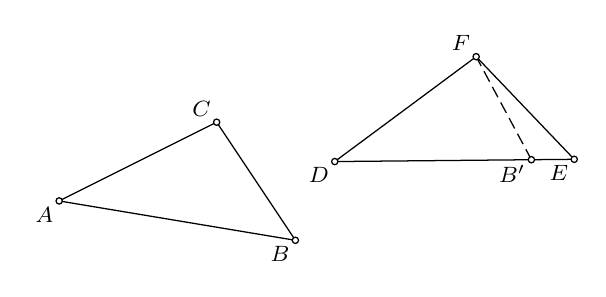
\begin{tikzpicture}
                % \clip (0,0) rectangle (14.000000,10.000000);
                {\footnotesize
                
                % Drawing segment A C
                \draw [line width=0.016cm] (1.535777,2.017889) -- (3.464223,2.982111);%
                
                % Drawing segment B C
                \draw [line width=0.016cm] (4.477812,1.533282) -- (3.522188,2.966718);%
                
                % Drawing segment A B
                \draw [line width=0.016cm] (1.539456,1.993424) -- (4.460544,1.506576);%
                
                % Drawing segment B' F
                \draw [line width=0.016cm] (7.478642,2.558692) -- (7.426668,2.655639);%
                \draw [line width=0.016cm] (7.391232,2.721739) -- (7.320359,2.853940);%
                \draw [line width=0.016cm] (7.284923,2.920041) -- (7.214050,3.052242);%
                \draw [line width=0.016cm] (7.178614,3.118342) -- (7.107741,3.250543);%
                \draw [line width=0.016cm] (7.072305,3.316643) -- (7.001432,3.448844);%
                \draw [line width=0.016cm] (6.965996,3.514945) -- (6.895123,3.647145);%
                \draw [line width=0.016cm] (6.859687,3.713246) -- (6.814867,3.796851);%
                
                % Drawing segment D E
                \draw [line width=0.016cm] (5.039998,2.500375) -- (7.457543,2.523063);%
                \draw [line width=0.016cm] (7.537539,2.523814) -- (8.001249,2.528165);%
                
                % Drawing segment D F
                \draw [line width=0.016cm] (5.032127,2.523829) -- (6.763840,3.808275);%
                
                % Drawing segment F E
                \draw [line width=0.016cm] (6.823598,3.803181) -- (8.013617,2.557464);%
                
                % Marking point A by circle
                \draw [line width=0.016cm] (1.500000,2.000000) circle (0.040000);%
                \draw (1.530000,2.030000) node [anchor=north east] { $A$ };%
                
                % Marking point B by circle
                \draw [line width=0.016cm] (4.500000,1.500000) circle (0.040000);%
                \draw (4.530000,1.530000) node [anchor=north east] { $B$ };%
                
                % Marking point C by circle
                \draw [line width=0.016cm] (3.500000,3.000000) circle (0.040000);%
                \draw (3.530000,2.970000) node [anchor=south east] { $C$ };%
                
                % Marking point D by circle
                \draw [line width=0.016cm] (5.000000,2.500000) circle (0.040000);%
                \draw (5.030000,2.530000) node [anchor=north east] { $D$ };%
                
                % Marking point E by circle
                \draw [line width=0.016cm] (8.041247,2.528541) circle (0.040000);%
                \draw (8.071247,2.558541) node [anchor=north east] { $E$ };%
                
                % Marking point B' by circle
                \draw [line width=0.016cm] (7.497541,2.523438) circle (0.040000);%
                \draw (7.527541,2.553438) node [anchor=north east] { $B'$ };%
                
                % Marking point F by circle
                \draw [line width=0.016cm] (6.795967,3.832104) circle (0.040000);%
                \draw (6.825967,3.802104) node [anchor=south east] { $F$ };%
                }
            \end{tikzpicture}
            \\ Uporabimo kriterij SKS. Primerjamo stranici $AB$ in $DE$. 
            Če velja $AB\cong DE$, po SKS sledi $\triangle ABC\cong \triangle DEF$.
            Denimo, da $AB\ncong DE$, torej je ena stranica krajša od druge, na primer je $AB<DE$. Tedaj obstaja točka $B'$, da je $D\ast B'\ast E$ in $AB\cong DB'$. Po SKS sledi: $\triangle CAB\cong\triangle FDB'$ ~ $\Rightarrow \angle DFB'\cong\angle ACB$ ($\cong DFE$ /po predpostavki/). Iz tega sledi: $\overrightarrow{FB'}=\overrightarrow{FE}$ $\Rightarrow B'=E$, to pa je protislovje ($AB<DE$).
        \end{dokaz}

    \begin{posledica}[I.6]
        Če v $\triangle ABC$ velja $\angle C\cong \angle B$, potem je $AC\cong BA$, torej je $\triangle ABC$ enakokrak.
    \end{posledica}

    \begin{trditev}[I.8 ali SSS]
        Če za $\triangle ABC$ in $\triangle DEF$ velja $AB\cong DE$, $BC\cong EF$ in $AC\cong DF$, potem je $\triangle ABC\cong \triangle DEF$.
    \end{trditev}

        \begin{dokaz}
            \\
            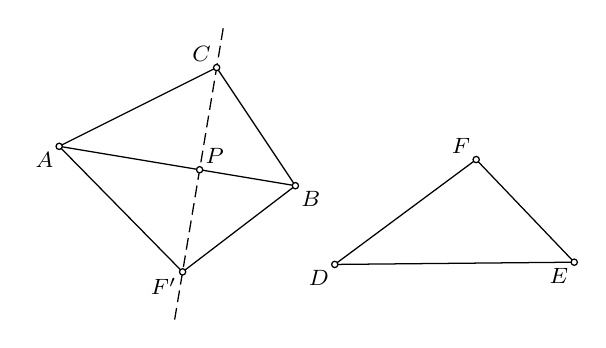
\begin{tikzpicture}
                % \clip (0,0) rectangle (14.000000,10.000000);
                {\footnotesize
                
                % Drawing line r
                \draw [line width=0.016cm] (2.966667,1.800000) -- (2.991327,1.947959);%
                \draw [line width=0.016cm] (3.003656,2.021939) -- (3.028316,2.169898);%
                \draw [line width=0.016cm] (3.040646,2.243877) -- (3.060992,2.365950);%
                \draw [line width=0.016cm] (3.077636,2.465816) -- (3.102296,2.613775);%
                \draw [line width=0.016cm] (3.114626,2.687755) -- (3.139286,2.835714);%
                \draw [line width=0.016cm] (3.151616,2.909693) -- (3.176275,3.057652);%
                \draw [line width=0.016cm] (3.188605,3.131632) -- (3.213265,3.279591);%
                \draw [line width=0.016cm] (3.225595,3.353570) -- (3.250255,3.501530);%
                \draw [line width=0.016cm] (3.262585,3.575509) -- (3.277208,3.663247);%
                \draw [line width=0.016cm] (3.299575,3.797448) -- (3.324234,3.945407);%
                \draw [line width=0.016cm] (3.336564,4.019386) -- (3.361224,4.167345);%
                \draw [line width=0.016cm] (3.373554,4.241325) -- (3.398214,4.389284);%
                \draw [line width=0.016cm] (3.410544,4.463264) -- (3.435204,4.611223);%
                \draw [line width=0.016cm] (3.447534,4.685202) -- (3.472194,4.833161);%
                \draw [line width=0.016cm] (3.484523,4.907141) -- (3.493424,4.960544);%
                \draw [line width=0.016cm] (3.506576,5.039456) -- (3.509183,5.055100);%
                \draw [line width=0.016cm] (3.521513,5.129079) -- (3.546173,5.277039);%
                \draw [line width=0.016cm] (3.558503,5.351018) -- (3.583163,5.498977);%
                
                % Drawing segment A C
                \draw [line width=0.016cm] (1.535777,4.017889) -- (3.464223,4.982111);%
                
                % Drawing segment B C
                \draw [line width=0.016cm] (4.477812,3.533282) -- (3.522188,4.966718);%
                
                % Drawing segment A B
                \draw [line width=0.016cm] (1.539456,3.993424) -- (3.244328,3.709279);%
                \draw [line width=0.016cm] (3.323240,3.696127) -- (4.460544,3.506576);%
                
                % Drawing segment D E
                \draw [line width=0.016cm] (5.039998,2.500375) -- (8.001249,2.528165);%
                
                % Drawing segment D F
                \draw [line width=0.016cm] (5.032127,2.523829) -- (6.763840,3.808275);%
                
                % Drawing segment F E
                \draw [line width=0.016cm] (6.823598,3.803181) -- (8.013617,2.557464);%
                
                % Drawing segment A F'
                \draw [line width=0.016cm] (1.528042,3.971475) -- (3.039526,2.433930);%
                
                % Drawing segment F' B
                \draw [line width=0.016cm] (3.099350,2.429692) -- (4.468217,3.475713);%
                
                % Marking point A by circle
                \draw [line width=0.016cm] (1.500000,4.000000) circle (0.040000);%
                \draw (1.530000,4.030000) node [anchor=north east] { $A$ };%
                
                % Marking point B by circle
                \draw [line width=0.016cm] (4.500000,3.500000) circle (0.040000);%
                \draw (4.470000,3.530000) node [anchor=north west] { $B$ };%
                
                % Marking point C by circle
                \draw [line width=0.016cm] (3.500000,5.000000) circle (0.040000);%
                \draw (3.530000,4.970000) node [anchor=south east] { $C$ };%
                
                % Marking point D by circle
                \draw [line width=0.016cm] (5.000000,2.500000) circle (0.040000);%
                \draw (5.030000,2.530000) node [anchor=north east] { $D$ };%
                
                % Marking point E by circle
                \draw [line width=0.016cm] (8.041247,2.528541) circle (0.040000);%
                \draw (8.071247,2.558541) node [anchor=north east] { $E$ };%
                
                % Marking point P by circle
                \draw [line width=0.016cm] (3.283784,3.702703) circle (0.040000);%
                \draw (3.253784,3.672703) node [anchor=south west] { $P$ };%
                
                % Marking point F by circle
                \draw [line width=0.016cm] (6.795967,3.832104) circle (0.040000);%
                \draw (6.825967,3.802104) node [anchor=south east] { $F$ };%
                
                % Marking point F' by circle
                \draw [line width=0.016cm] (3.067568,2.405405) circle (0.040000);%
                \draw (3.097568,2.435405) node [anchor=north east] { $F'$ };%
                }
            \end{tikzpicture}
            \\ Na nasprotnem bregu premice $\overleftrightarrow{AB}$ kot točka $C$ obstaja točka $F'$, da je $\triangle ABF'\cong \triangle DEF$.
            Opazimo, da sta trikotnika $\triangle CAF'$ in $\triangle CBF'$ enakokraka, z vrhom v $A$ oziroma v $B$. Zatorej sta kota ob osnovnici (v obeh trikotnikih) skladna. Ker je vsota skladnih kotov skladna, sledi, da je $\angle C\cong \angle F' (\cong \angle F)$. Zato po SKS sledi skladnost trikotnikov $\triangle ABC$ in $\triangle DEF$.
            \\ \uline{POZOR}: Možnih leg daljice $CF'$ glede na daljico $AB$ je več. Po konstrukciji sta točki $C$ in $F'$ na nasprotnih bregovih premice $\overleftrightarrow{AB}$, torej $CF'$ seka $\overleftrightarrow{AB}$ v neki točki $P$. Točka $P$ lahko leži med $A$ in $B$, lahko je eno od krajišč daljice $AB$ ali pa leži izven daljice $AB$. V slednjem primeru uporabimo dejstvo, da je razlika skladnih kotov skladna.
            \\
            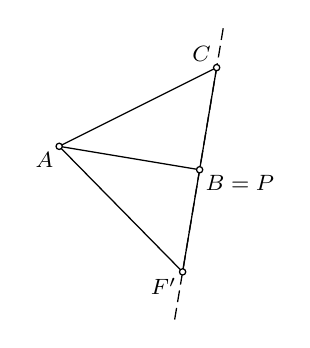
\begin{tikzpicture}
                % \clip (0,0) rectangle (14.000000,10.000000);
                {\footnotesize
                
                % Drawing line r
                \draw [line width=0.016cm] (2.966667,1.800000) -- (2.991327,1.947959);%
                \draw [line width=0.016cm] (3.003656,2.021939) -- (3.028316,2.169898);%
                \draw [line width=0.016cm] (3.040646,2.243877) -- (3.060992,2.365950);%
                \draw [line width=0.016cm] (3.077636,2.465816) -- (3.102296,2.613775);%
                \draw [line width=0.016cm] (3.114626,2.687755) -- (3.139286,2.835714);%
                \draw [line width=0.016cm] (3.151616,2.909693) -- (3.176275,3.057652);%
                \draw [line width=0.016cm] (3.188605,3.131632) -- (3.213265,3.279591);%
                \draw [line width=0.016cm] (3.225595,3.353570) -- (3.250255,3.501530);%
                \draw [line width=0.016cm] (3.262585,3.575509) -- (3.277208,3.663247);%
                \draw [line width=0.016cm] (3.299575,3.797448) -- (3.324234,3.945407);%
                \draw [line width=0.016cm] (3.336564,4.019386) -- (3.361224,4.167345);%
                \draw [line width=0.016cm] (3.373554,4.241325) -- (3.398214,4.389284);%
                \draw [line width=0.016cm] (3.410544,4.463264) -- (3.435204,4.611223);%
                \draw [line width=0.016cm] (3.447534,4.685202) -- (3.472194,4.833161);%
                \draw [line width=0.016cm] (3.484523,4.907141) -- (3.493424,4.960544);%
                \draw [line width=0.016cm] (3.506576,5.039456) -- (3.509183,5.055100);%
                \draw [line width=0.016cm] (3.521513,5.129079) -- (3.546173,5.277039);%
                \draw [line width=0.016cm] (3.558503,5.351018) -- (3.583163,5.498977);%
                
                % Drawing segment A C
                \draw [line width=0.016cm] (1.535777,4.017889) -- (3.464223,4.982111);%
                
                % Drawing segment A B=D
                \draw [line width=0.016cm] (1.539456,3.993424) -- (3.244328,3.709279);%
                
                % Drawing segment A F'
                \draw [line width=0.016cm] (1.528042,3.971475) -- (3.039526,2.433930);%
                
                % Drawing segment C F'
                \draw [line width=0.016cm] (3.493424,4.960544) -- (3.290360,3.742158);%
                \draw [line width=0.016cm] (3.277208,3.663247) -- (3.074144,2.444861);%
                
                % Marking point A by circle
                \draw [line width=0.016cm] (1.500000,4.000000) circle (0.040000);%
                \draw (1.530000,4.030000) node [anchor=north east] { $A$ };%
                
                % Marking point B=D by circle
                \draw [line width=0.016cm] (3.283784,3.702703) circle (0.040000);%
                \draw (3.253784,3.732703) node [anchor=north west] { $B=P$ };%
                
                % Marking point C by circle
                \draw [line width=0.016cm] (3.500000,5.000000) circle (0.040000);%
                \draw (3.530000,4.970000) node [anchor=south east] { $C$ };%
                
                % Marking point F' by circle
                \draw [line width=0.016cm] (3.067568,2.405405) circle (0.040000);%
                \draw (3.097568,2.435405) node [anchor=north east] { $F'$ };%
                }
            \end{tikzpicture}
            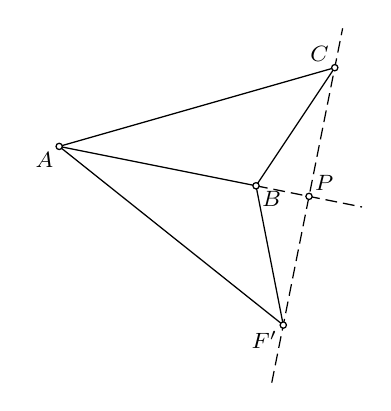
\begin{tikzpicture}
                % \clip (0,0) rectangle (14.000000,10.000000);
                {\footnotesize
                
                % Drawing line r
                \draw [line width=0.016cm] (4.200000,1.000000) -- (4.229417,1.147087);%
                \draw [line width=0.016cm] (4.244126,1.220631) -- (4.273544,1.367718);%
                \draw [line width=0.016cm] (4.288252,1.441261) -- (4.317670,1.588348);%
                \draw [line width=0.016cm] (4.332378,1.661892) -- (4.338309,1.691546);%
                \draw [line width=0.016cm] (4.353998,1.769992) -- (4.361796,1.808979);%
                \draw [line width=0.016cm] (4.376505,1.882523) -- (4.405922,2.029610);%
                \draw [line width=0.016cm] (4.420631,2.103153) -- (4.450048,2.250240);%
                \draw [line width=0.016cm] (4.464757,2.323784) -- (4.494174,2.470871);%
                \draw [line width=0.016cm] (4.508883,2.544415) -- (4.538300,2.691502);%
                \draw [line width=0.016cm] (4.553009,2.765045) -- (4.582426,2.912132);%
                \draw [line width=0.016cm] (4.597135,2.985676) -- (4.626553,3.132763);%
                \draw [line width=0.016cm] (4.641261,3.206307) -- (4.665232,3.326161);%
                \draw [line width=0.016cm] (4.685387,3.426937) -- (4.714805,3.574024);%
                \draw [line width=0.016cm] (4.729514,3.647568) -- (4.758931,3.794655);%
                \draw [line width=0.016cm] (4.773640,3.868198) -- (4.803057,4.015286);%
                \draw [line width=0.016cm] (4.817766,4.088829) -- (4.847183,4.235916);%
                \draw [line width=0.016cm] (4.861892,4.309460) -- (4.891309,4.456547);%
                \draw [line width=0.016cm] (4.906018,4.530090) -- (4.935436,4.677178);%
                \draw [line width=0.016cm] (4.950144,4.750721) -- (4.979562,4.897808);%
                \draw [line width=0.016cm] (5.007845,5.039223) -- (5.023688,5.118439);%
                \draw [line width=0.016cm] (5.038396,5.191982) -- (5.067814,5.339069);%
                \draw [line width=0.016cm] (5.082523,5.412613) -- (5.100000,5.500000);%
                
                % Drawing segment A C
                \draw [line width=0.016cm] (1.538461,4.010989) -- (4.961539,4.989011);%
                
                % Drawing segment B C
                \draw [line width=0.016cm] (4.022188,3.533282) -- (4.977812,4.966718);%
                
                % Drawing segment A B
                \draw [line width=0.016cm] (1.539223,3.992155) -- (3.960777,3.507845);%
                
                % Drawing segment A F'
                \draw [line width=0.016cm] (1.531276,3.975064) -- (4.314878,1.755705);%
                
                % Drawing segment F' B
                \draw [line width=0.016cm] (4.338473,1.770025) -- (4.007680,3.460744);%
                
                % Drawing segment B P'
                \draw [line width=0.016cm] (4.039223,3.492155) -- (4.147087,3.470583);%
                \draw [line width=0.016cm] (4.220631,3.455874) -- (4.367718,3.426456);%
                \draw [line width=0.016cm] (4.441261,3.411748) -- (4.588348,3.382330);%
                \draw [line width=0.016cm] (4.712300,3.357540) -- (4.808979,3.338204);%
                \draw [line width=0.016cm] (4.882523,3.323495) -- (5.029610,3.294078);%
                \draw [line width=0.016cm] (5.103153,3.279369) -- (5.250240,3.249952);%
                \draw [line width=0.016cm] (5.323784,3.235243) -- (5.346154,3.230769);%
                
                % Marking point A by circle
                \draw [line width=0.016cm] (1.500000,4.000000) circle (0.040000);%
                \draw (1.530000,4.030000) node [anchor=north east] { $A$ };%
                
                % Marking point B by circle
                \draw [line width=0.016cm] (4.000000,3.500000) circle (0.040000);%
                \draw (3.970000,3.530000) node [anchor=north west] { $B$ };%
                
                % Marking point C by circle
                \draw [line width=0.016cm] (5.000000,5.000000) circle (0.040000);%
                \draw (5.030000,4.970000) node [anchor=south east] { $C$ };%
                
                % Marking point P by circle
                \draw [line width=0.016cm] (4.673077,3.365385) circle (0.040000);%
                \draw (4.643077,3.335385) node [anchor=south west] { $P$ };%
                
                % Marking point F' by circle
                \draw [line width=0.016cm] (4.346154,1.730769) circle (0.040000);%
                \draw (4.376154,1.760769) node [anchor=north east] { $F'$ };%
                }
            \end{tikzpicture}    
        \end{dokaz}

    \begin{trditev}
        Vsi pravi koti so skladni.
    \end{trditev}

        \begin{dokaz}
            \\
            \begin{tikzpicture}
                % \clip (0,0) rectangle (14.000000,10.000000);
                {\footnotesize
                
                % Marking point A by circle
                \draw [line width=0.016cm] (3.000000,1.500000) circle (0.040000);%
                \draw (3.030000,1.530000) node [anchor=north east] { $A$ };%
                
                % Marking point B by circle
                \draw [line width=0.016cm] (4.000000,1.500000) circle (0.040000);%
                \draw (4.030000,1.530000) node [anchor=north east] { $B$ };%
                
                % Marking point D by circle
                \draw [line width=0.016cm] (1.500000,1.500000) circle (0.040000);%
                \draw (1.530000,1.530000) node [anchor=north east] { $D$ };%
                
                % Marking point C by circle
                \draw [line width=0.016cm] (3.000000,3.000000) circle (0.040000);%
                \draw (3.030000,2.970000) node [anchor=south east] { $C$ };%
                
                % Drawing segment H I
                \draw [line width=0.016cm] (1.000000,1.500000) -- (1.460000,1.500000);%
                \draw [line width=0.016cm] (1.540000,1.500000) -- (2.960000,1.500000);%
                \draw [line width=0.016cm] (3.040000,1.500000) -- (3.960000,1.500000);%
                \draw [line width=0.016cm] (4.040000,1.500000) -- (4.500000,1.500000);%
                
                % Drawing line r
                \draw [line width=0.016cm] (3.000000,1.000000) -- (3.000000,1.460000);%
                \draw [line width=0.016cm] (3.000000,1.540000) -- (3.000000,2.960000);%
                \draw [line width=0.016cm] (3.000000,3.040000) -- (3.000000,3.500000);%
                
                % Marking point A' by circle
                \draw [line width=0.016cm] (7.000000,1.500000) circle (0.040000);%
                \draw (7.030000,1.530000) node [anchor=north east] { $A'$ };%
                
                % Marking point B' by circle
                \draw [line width=0.016cm] (8.000000,1.500000) circle (0.040000);%
                \draw (8.030000,1.530000) node [anchor=north east] { $B'$ };%
                
                % Marking point D' by circle
                \draw [line width=0.016cm] (5.500000,1.500000) circle (0.040000);%
                \draw (5.530000,1.530000) node [anchor=north east] { $D'$ };%
                
                % Marking point C' by circle
                \draw [line width=0.016cm] (7.000000,3.000000) circle (0.040000);%
                \draw (7.030000,2.970000) node [anchor=south east] { $C'$ };%
                
                % Marking point C'' by circle
                \draw [line width=0.016cm] (7.500000,2.700000) circle (0.040000);%
                \draw (7.530000,2.670000) node [anchor=south east] { $C''$ };%
                
                % Drawing segment H' I'
                \draw [line width=0.016cm] (5.000000,1.500000) -- (5.460000,1.500000);%
                \draw [line width=0.016cm] (5.540000,1.500000) -- (6.960000,1.500000);%
                \draw [line width=0.016cm] (7.040000,1.500000) -- (7.960000,1.500000);%
                \draw [line width=0.016cm] (8.040000,1.500000) -- (8.500000,1.500000);%
                
                % Drawing line r'
                \draw [line width=0.016cm] (7.000000,1.000000) -- (7.000000,1.460000);%
                \draw [line width=0.016cm] (7.000000,1.540000) -- (7.000000,2.960000);%
                \draw [line width=0.016cm] (7.000000,3.040000) -- (7.000000,3.500000);%
                
                % Drawing segment A' G'
                \draw [line width=0.016cm] (7.015385,1.536923) -- (7.484615,2.663077);%
                \draw [line width=0.016cm] (7.515385,2.736923) -- (7.750000,3.300000);%
                }
            \end{tikzpicture}
            \\ Naj bosta $\angle BAC$ in $\angle B'A'C'$ prava kota. Recimo, da $\angle BAC \ncong\angle B'A'C'$, npr. $\angle BAC < \angle B'A'C'$.
            Potem obstaja točka $C''$ znotraj $\angle B'A'C'$, da je $\angle BAC\cong\angle B'A'C''$. Ker so suplementarni koti skladnih kotov skladni, je $\angle DAC\cong \angle D'A'C''$.
            Sledi: $\angle BAC \cong \angle B'A'C'' < \angle B'A'C' \cong \angle D'A'C' < \angle D'A'C'' \cong \angle DAC \cong \angle BAC$, kar pa je protislovje, saj kot ne more biti manjši od samega sebe.
        \end{dokaz}

\section{Aksiomi zveznosti}

    \begin{aksiom}[Dedekind]
        Naj bo množica točk na premici $p$ disjunktna unija dveh nepraznih podmnožic $\Sigma_1$ in $\Sigma_2$, za kateri velja: nobena točka v $\Sigma_1$ ($\Sigma_2$) ne leži med dvema točkama v $\Sigma_2$ ($\Sigma_1$).
        Potem obstaja natanko ena točka $A$ na $p$, da je ena od množic $\Sigma_1$ in $\Sigma_2$ enaka enemu od poltrakov na $p$ z začetkom v $A$, druga pa je komplement tega poltraka.
    \end{aksiom}

        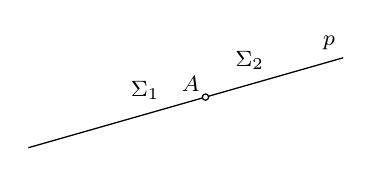
\begin{tikzpicture}
            % \clip (0,0) rectangle (14.000000,10.000000);
            {\footnotesize
            
            % Drawing line q p
            \draw [line width=0.016cm] (1.000000,1.357143) -- (3.211539,1.989011);%
            \draw [line width=0.016cm] (3.288461,2.010989) -- (5.000000,2.500000);%
            
            % Marking point p
            \draw (5.000000,2.500000) node [anchor=south east] { $p$ };%
            
            % Marking point \Sigma_1
            \draw (2.771363,1.863247) node [anchor=south east] { $\Sigma_1$ };%
            
            % Marking point A by circle
            \draw [line width=0.016cm] (3.250000,2.000000) circle (0.040000);%
            \draw (3.280000,1.970000) node [anchor=south east] { $A$ };%
            
            % Marking point \Sigma_2
            \draw (4.098643,2.242470) node [anchor=south east] { $\Sigma_2$ };%
            }
        \end{tikzpicture}
        

        Enako kot v $\RR$: množica točk na premici je polna, tj. vedno obstaja delilna točka ($A$) med $\Sigma_1$ in $\Sigma_2$. Torej je vsaka premica kopija $\RR$.
        \\
        \\
        Na osnovi Dedekindovega aksioma lahko v ravnino vpeljemo koordinate in delamo geometrijo analitično. (Descartes in Fermat v 17. stoletju)
        \\
        \\
        \underline{Motivacija}: Evklidov dokaz I.1: konstrukcija enakostraničnega trikotnika na dani daljici:
         Narišemo krožnico s središčem v $A$ in polmerom $AB$ in krožnico s središčem v $B$ in polmerom $BA$. Presečišče $C$ teh krožnic da tretje oglišče enakostraničnega trikotnika.
        \\
        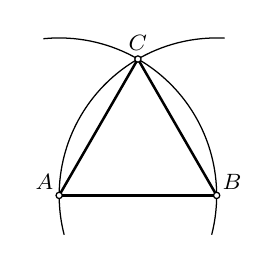
\begin{tikzpicture}
            % \clip (0,0) rectangle (14.000000,10.000000);
            {\footnotesize
            
            % Drawing circle k1
            \draw [line width=0.016cm] (3.999600,1.539998) -- (3.998782,1.569799) arc (2:58:2.000000 and 2.000000) -- (3.034439,3.211705);%
            \draw [line width=0.016cm] (2.965161,3.251703) -- (2.938943,3.265895) arc (62:95:2.000000 and 2.000000) -- (1.800000,3.489975);%
            \draw [line width=0.016cm] (3.936492,0.999999) -- (3.940591,1.016156) arc (346:358:2.000000 and 2.000000) -- (3.999600,1.460001);%
            
            % Drawing circle k2
            \draw [line width=0.016cm] (4.100000,3.497498) -- (4.069799,3.498782) arc (88:118:2.000000 and 2.000000) -- (3.034839,3.251703);%
            \draw [line width=0.016cm] (2.965561,3.211705) -- (2.940162,3.196096) arc (122:178:2.000000 and 2.000000) -- (2.000400,1.539998);%
            \draw [line width=0.016cm] (2.000400,1.460003) -- (2.001218,1.430201) arc (182:194:2.000000 and 2.000000) -- (2.063508,1.000001);%
            
            % Marking point A by circle
            \draw [line width=0.016cm] (2.000000,1.500000) circle (0.040000);%
            \draw (2.030000,1.470000) node [anchor=south east] { $A$ };%
            
            % Marking point B by circle
            \draw [line width=0.016cm] (4.000000,1.500000) circle (0.040000);%
            \draw (3.970000,1.470000) node [anchor=south west] { $B$ };%
            
            % Marking point C by circle
            \draw [line width=0.016cm] (3.000000,3.232051) circle (0.040000);%
            \draw (3.000000,3.232051) node [anchor=south] { $C$ };%
            
            % Drawing segment A B
            \draw [line width=0.032cm] (2.040000,1.500000) -- (3.960000,1.500000);%
            
            % Drawing segment A C
            \draw [line width=0.032cm] (2.020000,1.534641) -- (2.980000,3.197410);%
            
            % Drawing segment B C
            \draw [line width=0.032cm] (3.980000,1.534641) -- (3.020000,3.197410);%
            }
        \end{tikzpicture}
        \\ \underline{Težava}: Iz aksiomov ni mogoče izpeljati, da se krožnici sekata. --- Privzamemo lahko aksiom o zveznosti krožnic.
    
    \begin{aksiom}[Zveznost krožnic]
        Če ima krožnica $\delta$ eno točko \textit{znotraj} in eno točko \textit{zunaj} krožnice $\delta'$, potem se krožnici sekata v dveh točkah.
    \end{aksiom}

        Pri zveznosti krožnic obstaja tudi šibkejši aksiom, ki zagotavlja, da daljica, ki ima eno krajišče znotraj krožnice in drugo izven, to krožnico seka.

        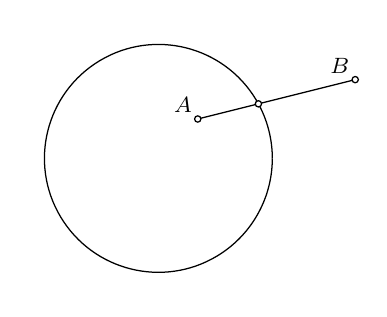
\begin{tikzpicture}
            % \clip (0,0) rectangle (14.000000,10.000000);
            {\footnotesize
            
            % Drawing circle k
            \draw [line width=0.016cm] (3.947002,2.500000) arc (0:27:1.447002 and 1.447002) -- (3.789129,3.157236);%
            \draw [line width=0.016cm] (3.750840,3.227470) -- (3.740323,3.245261) arc (31:359:1.447002 and 1.447002) -- (3.947002,2.500000);%
            
            % Drawing segment A B
            \draw [line width=0.016cm] (3.038806,3.009701) -- (3.731665,3.182916);%
            \draw [line width=0.016cm] (3.809276,3.202319) -- (4.961194,3.490299);%
            
            % Marking point P by circle
            \draw [line width=0.016cm] (3.770470,3.192618) circle (0.040000);%
            
            % Marking point A by circle
            \draw [line width=0.016cm] (3.000000,3.000000) circle (0.040000);%
            \draw (3.030000,2.970000) node [anchor=south east] { $A$ };%
            
            % Marking point B by circle
            \draw [line width=0.016cm] (5.000000,3.500000) circle (0.040000);%
            \draw (5.030000,3.470000) node [anchor=south east] { $B$ };%
            }
        \end{tikzpicture}

    \begin{aksiom}[Arhimed]
        Naj bo $CD$ poljubna daljica, $A$ poljubna točka in $r$ poltrak z začetkom v $A$.
        Potem za poljubno točko $B\neq A$ na $r$ obstaja naravno število $n$ z lastnostjo: če na poltraku $r$ odmerimo $n$ kopij daljice $CD$ z začetkom v $A$, potem dobimo točko $E$, za katero velja $n*CD\cong AE$ in bodisi $B=E$ bodisi $A\ast B\ast E$.
    \end{aksiom}

        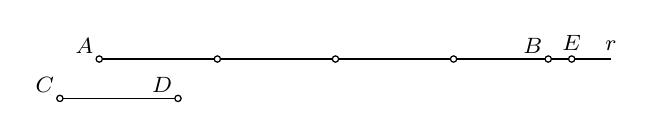
\begin{tikzpicture}
            % \clip (0,0) rectangle (14.000000,10.000000);
            {\footnotesize
            
            % Drawing segment A X
            \draw [line width=0.016cm] (2.040000,2.000000) -- (3.460000,2.000000);%
            \draw [line width=0.016cm] (3.540000,2.000000) -- (4.960000,2.000000);%
            \draw [line width=0.016cm] (5.040000,2.000000) -- (6.460000,2.000000);%
            \draw [line width=0.016cm] (6.540000,2.000000) -- (7.662155,2.000000);%
            \draw [line width=0.016cm] (7.742155,2.000000) -- (7.960000,2.000000);%
            \draw [line width=0.016cm] (8.040000,2.000000) -- (8.500000,2.000000);%
            
            % Drawing segment C D
            \draw [line width=0.016cm] (1.540000,1.500000) -- (2.960000,1.500000);%
            
            % Marking point A by circle
            \draw [line width=0.016cm] (2.000000,2.000000) circle (0.040000);%
            \draw (2.030000,1.970000) node [anchor=south east] { $A$ };%
            
            % Marking point B by circle
            \draw [line width=0.016cm] (7.702155,2.000000) circle (0.040000);%
            \draw (7.732155,1.970000) node [anchor=south east] { $B$ };%
            
            % Marking point C by circle
            \draw [line width=0.016cm] (1.500000,1.500000) circle (0.040000);%
            \draw (1.530000,1.470000) node [anchor=south east] { $C$ };%
            
            % Marking point D by circle
            \draw [line width=0.016cm] (3.000000,1.500000) circle (0.040000);%
            \draw (3.030000,1.470000) node [anchor=south east] { $D$ };%
            
            % Marking point D' by circle
            \draw [line width=0.016cm] (3.500000,2.000000) circle (0.040000);%
            
            % Marking point D'' by circle
            \draw [line width=0.016cm] (5.000000,2.000000) circle (0.040000);%
            
            % Marking point D''' by circle
            \draw [line width=0.016cm] (6.500000,2.000000) circle (0.040000);%
            
            % Marking point D'''' by circle
            \draw [line width=0.016cm] (8.000000,2.000000) circle (0.040000);%
            \draw (8.000000,2.00000) node [anchor=south] { $E$ };%

            % Marking point r
            \draw (8.50000,2.000000) node [anchor=south] { $r$ };%
            
            }
        \end{tikzpicture}

        Ta aksiom govori o primerljivosti 'dolžin' (velikosti) daljic, tj. ni neprimerljivo velikih daljic. To je v $\RR$ zajeto v Arhimedski lastnosti.

    \begin{aksiom}[Aristotel]
        Za izbrano stranico/krak $r$ poljubnega ostrega kota in poljubno daljico $AB$ obstaja točka $C$ na $r$, da velja: če je $D$ nožišče pravokotnice iz $C$ na drugo stranico/krak kota, potem je $CD>AB$.
    \end{aksiom}

        \begin{tikzpicture}
            % \clip (0,0) rectangle (14.000000,10.000000);
            {\footnotesize
            
            % Marking point A by circle
            \draw [line width=0.016cm] (1.500000,1.500000) circle (0.040000);%
            \draw (1.530000,1.470000) node [anchor=south east] { $A$ };%
            
            % Marking point B by circle
            \draw [line width=0.016cm] (2.000000,2.500000) circle (0.040000);%
            \draw (2.030000,2.470000) node [anchor=south east] { $B$ };%
            
            % Marking point r
            \draw (7.000000,2.000000) node [anchor=south east] { $r$ };%
            
            % Marking point C by circle
            \draw [line width=0.016cm] (6.177374,2.000000) circle (0.040000);%
            \draw (6.207374,1.970000) node [anchor=south east] { $C$ };%
            
            % Marking point D by circle
            \draw [line width=0.016cm] (5.570796,3.364798) circle (0.040000);%
            \draw (5.600796,3.334798) node [anchor=south east] { $D$ };%
            
            % Drawing segment X r
            \draw [line width=0.016cm] (2.500000,2.000000) -- (6.137374,2.000000);%
            \draw [line width=0.016cm] (6.217374,2.000000) -- (7.000000,2.000000);%
            
            % Drawing segment X q
            \draw [line width=0.016cm] (2.500000,2.000000) -- (5.534244,3.348553);%
            \draw [line width=0.016cm] (5.607349,3.381044) -- (7.000000,4.000000);%
            
            % Drawing segment C D
            \draw [line width=0.016cm] (6.161128,2.036552) -- (5.587042,3.328246);%
            
            % Drawing segment A B
            \draw [line width=0.016cm] (1.517889,1.535777) -- (1.982111,2.464223);%
            }
        \end{tikzpicture}
        

\section{Aksiomi vzporednosti}

    \begin{aksiom}[Hilbertov aksiom o vzporednicah]
        Za vsako premico $p$ in vsako točko $A$, ki ne leži na $p$, obstaja natanko ena premica $q$ skozi $A$, ki je vzporedna $p$.
    \end{aksiom}

        \begin{tikzpicture}
            % \clip (0,0) rectangle (14.000000,10.000000);
            {\footnotesize
            
            % Marking point A by circle
            \draw [line width=0.016cm] (3.000000,3.000000) circle (0.040000);%
            \draw (3.030000,2.970000) node [anchor=south east] { $A$ };%
            
            % Marking point p
            \draw (5.000000,2.000000) node [anchor=south east] { $p$ };%
            
            % Marking point q
            \draw (5.000000,3.300000) node [anchor=south east] { $q$ };%
            
            % Drawing line P
            \draw [line width=0.016cm] (1.000000,1.428571) -- (1.148492,1.449785);%
            \draw [line width=0.016cm] (1.222739,1.460391) -- (1.371231,1.481604);%
            \draw [line width=0.016cm] (1.445477,1.492211) -- (1.593970,1.513424);%
            \draw [line width=0.016cm] (1.668216,1.524031) -- (1.816708,1.545244);%
            \draw [line width=0.016cm] (1.890955,1.555851) -- (2.039447,1.577064);%
            \draw [line width=0.016cm] (2.113693,1.587670) -- (2.262186,1.608884);%
            \draw [line width=0.016cm] (2.336432,1.619490) -- (2.484924,1.640703);%
            \draw [line width=0.016cm] (2.559170,1.651310) -- (2.707663,1.672523);%
            \draw [line width=0.016cm] (2.781909,1.683130) -- (2.930402,1.704343);%
            \draw [line width=0.016cm] (3.004648,1.714950) -- (3.153140,1.736163);%
            \draw [line width=0.016cm] (3.227386,1.746769) -- (3.375879,1.767983);%
            \draw [line width=0.016cm] (3.450125,1.778589) -- (3.598617,1.799802);%
            \draw [line width=0.016cm] (3.672864,1.810409) -- (3.821356,1.831622);%
            \draw [line width=0.016cm] (3.895602,1.842229) -- (4.044095,1.863442);%
            \draw [line width=0.016cm] (4.118341,1.874049) -- (4.266833,1.895262);%
            \draw [line width=0.016cm] (4.341080,1.905869) -- (4.489572,1.927082);%
            \draw [line width=0.016cm] (4.563818,1.937688) -- (4.712311,1.958902);%
            \draw [line width=0.016cm] (4.786557,1.969508) -- (4.935049,1.990721);%
            
            % Drawing line Q
            \draw [line width=0.016cm] (1.000000,2.714286) -- (2.960402,2.994343);%
            \draw [line width=0.016cm] (3.039598,3.005657) -- (5.000000,3.285714);%
            }
        \end{tikzpicture}

    \begin{aksiom}[Evklidov 5. aksiom]
        Če premici $p$ in $q$ seka premica $t$ tako, da vsota notranjih kotov na enem bregu $t$ meri manj kot $\pi$, potem se premici $p$ in $q$ sekata na tem bregu $t$.
    \end{aksiom}

        \begin{tikzpicture}
            % \clip (0,0) rectangle (14.000000,10.000000);
            {\footnotesize
            
            % Drawing line T
            \draw [line width=0.016cm] (1.666667,1.000000) -- (2.666667,4.000000);%
            
            % Drawing line Q
            \draw [line width=0.016cm] (1.000000,3.500000) -- (6.245714,3.500000);%
            \draw [line width=0.016cm] (6.325714,3.500000) -- (7.000000,3.500000);%
            
            % Drawing line P
            \draw [line width=0.016cm] (1.000000,1.650000) -- (6.247960,3.486786);%
            \draw [line width=0.016cm] (6.323469,3.513214) -- (7.000000,3.750000);%
            
            % Marking point q
            \draw (4.000000,3.500000) node [anchor=south east] { $q$ };%
            
            % Marking point p
            \draw (4.000000,2.700000) node [anchor=south east] { $p$ };%
            
            % Marking point \alpha
            \draw (2.500000,3.500000) node [anchor=north west] { $\alpha$ };%
            
            % Marking point \beta
            \draw (2.000000,2.000000) node [anchor=south west] { $\beta$ };%
            
            % Marking point W by circle
            \draw [line width=0.016cm] (6.285714,3.500000) circle (0.040000);%
            
            % Marking point t
            \draw (2.262368,2.787103) node [anchor=south east] { $t$ };%
            }
        \end{tikzpicture}
        
    \begin{aksiom}[Hiperbolični aksiom o vzporednicah]
        Obstaja premica $p$ in točka $A$, ki ne leži na $p$, da skozi $A$ potekata vsaj dve vzporednici k $p$.
    \end{aksiom}

        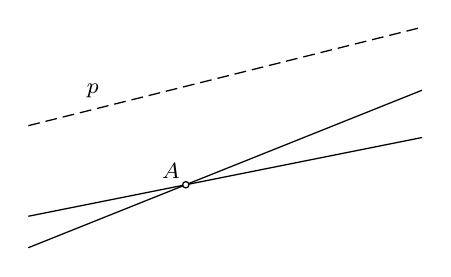
\begin{tikzpicture}
            % \clip (0,0) rectangle (14.000000,10.000000);
            {\footnotesize
            
            % Drawing line p X
            \draw [line width=0.016cm] (1.000000,3.250000) -- (1.145521,3.286380);%
            \draw [line width=0.016cm] (1.218282,3.304571) -- (1.363803,3.340951);%
            \draw [line width=0.016cm] (1.436564,3.359141) -- (1.582086,3.395521);%
            \draw [line width=0.016cm] (1.654846,3.413712) -- (1.800368,3.450092);%
            \draw [line width=0.016cm] (1.873128,3.468282) -- (2.018650,3.504662);%
            \draw [line width=0.016cm] (2.091410,3.522853) -- (2.236932,3.559233);%
            \draw [line width=0.016cm] (2.309692,3.577423) -- (2.455214,3.613803);%
            \draw [line width=0.016cm] (2.527974,3.631994) -- (2.673496,3.668374);%
            \draw [line width=0.016cm] (2.746257,3.686564) -- (2.891778,3.722944);%
            \draw [line width=0.016cm] (2.964539,3.741135) -- (3.110060,3.777515);%
            \draw [line width=0.016cm] (3.182821,3.795705) -- (3.328342,3.832086);%
            \draw [line width=0.016cm] (3.401103,3.850276) -- (3.546624,3.886656);%
            \draw [line width=0.016cm] (3.619385,3.904846) -- (3.764906,3.941227);%
            \draw [line width=0.016cm] (3.837667,3.959417) -- (3.983188,3.995797);%
            \draw [line width=0.016cm] (4.055949,4.013987) -- (4.201470,4.050368);%
            \draw [line width=0.016cm] (4.274231,4.068558) -- (4.419752,4.104938);%
            \draw [line width=0.016cm] (4.492513,4.123128) -- (4.638034,4.159509);%
            \draw [line width=0.016cm] (4.710795,4.177699) -- (4.856316,4.214079);%
            \draw [line width=0.016cm] (4.929077,4.232269) -- (5.074599,4.268650);%
            \draw [line width=0.016cm] (5.147359,4.286840) -- (5.292881,4.323220);%
            \draw [line width=0.016cm] (5.365641,4.341410) -- (5.511163,4.377791);%
            \draw [line width=0.016cm] (5.583923,4.395981) -- (5.729445,4.432361);%
            \draw [line width=0.016cm] (5.802205,4.450551) -- (5.947727,4.486932);%
            
            % Drawing line A Y
            \draw [line width=0.016cm] (1.000000,2.100000) -- (2.960777,2.492155);%
            \draw [line width=0.016cm] (3.039223,2.507845) -- (6.000000,3.100000);%
            
            % Drawing line A Z
            \draw [line width=0.016cm] (1.000000,1.700000) -- (2.962861,2.485144);%
            \draw [line width=0.016cm] (3.037139,2.514856) -- (6.000000,3.700000);%
            
            % Marking point A by circle
            \draw [line width=0.016cm] (3.000000,2.500000) circle (0.040000);%
            \draw (3.030000,2.470000) node [anchor=south east] { $A$ };%
            
            % Marking point p
            \draw (2.000000,3.500000) node [anchor=south east] { $p$ };%
            }
        \end{tikzpicture}
        
